\documentclass[aspectratio=169,11pt]{beamer}
\usetheme{metropolis}
\usepackage{tikz}
\usetikzlibrary{arrows.meta,positioning,decorations.pathmorphing,calc,shapes.geometric,decorations.pathreplacing,patterns}
\usepackage{pgfplots}
\pgfplotsset{compat=1.18}
\usepackage{booktabs}
\usepackage{xcolor}
\usepackage{amsmath,amssymb}
\usepackage{graphicx}
\graphicspath{{figures/generated/}}
\usepackage{hyperref}
\hypersetup{colorlinks=true,urlcolor=grass,linkcolor=black,citecolor=black}
\usepackage{multirow}

\definecolor{grass}{HTML}{2E7D32}
\definecolor{circle}{HTML}{E91E63}
\definecolor{das}{HTML}{2196F3}
\definecolor{vae}{HTML}{9C27B0}
\definecolor{nldas}{HTML}{FF9800}
\definecolor{neutral}{HTML}{9E9E9E}
\definecolor{pass}{HTML}{4CAF50}
\definecolor{fail}{HTML}{F44336}
\definecolor{stoch}{HTML}{FF9800}
\definecolor{never}{HTML}{F44336}
\definecolor{always}{HTML}{4CAF50}
\definecolor{bg}{HTML}{FAFAFA}
\definecolor{memo}{HTML}{795548}

\newcommand{\Gr}{\mathrm{Gr}}
\newcommand{\IIA}{\mathrm{IIA}}
\newcommand{\R}{\mathbb{R}}
\newcommand{\Z}{\mathbb{Z}}

\title{Learning Causal Variables, Not Causal Directions}
\subtitle{Structured sparse autoencoders for nonlinear causal discovery\\[0.3em]{\small Validated on 5 GPT-2 tasks from the MIB benchmark}}
\author{Elliot Tower}
\date{2026}
\institute{}

\begin{document}

\maketitle

%% --- OVERVIEW ---
\begin{frame}{Overview}
\begin{columns}[T]
\begin{column}{0.32\textwidth}
\textbf{\hyperlink{part1}{Part 1: Setup}}
\begin{enumerate}
  \item \hyperlink{sec1}{What is a causal variable?}
  \item \hyperlink{sec2}{DAS and the Grassmannian}
  \item \hyperlink{sec3}{Why linearity matters}
\end{enumerate}
\vspace{0.5em}
\textbf{\hyperlink{part2}{Part 2: The atlas}}
\begin{enumerate}
  \setcounter{enumi}{3}
  \item \hyperlink{sec4}{14 operations, three classes}
  \item \hyperlink{sec5}{Linear DAS fails completely}
  \item \hyperlink{sec6}{Stochastic grokking}
\end{enumerate}
\end{column}
\begin{column}{0.32\textwidth}
\textbf{\hyperlink{part3}{Part 3: The vacuity problem}}
\begin{enumerate}
  \setcounter{enumi}{6}
  \item \hyperlink{sec7}{Memorization artifacts}
  \item \hyperlink{sec8}{Nonlinear DAS is vacuous}
  \item \hyperlink{sec9}{Intervention faithfulness}
\end{enumerate}
\vspace{0.5em}
\textbf{\hyperlink{part4}{Part 4: The fix}}
\begin{enumerate}
  \setcounter{enumi}{9}
  \item \hyperlink{sec10}{Structured VAE}
  \item \hyperlink{sec11}{Cross-task transfer}
  \item \hyperlink{sec12}{IOI is not Grassmannian}
\end{enumerate}
\end{column}
\begin{column}{0.32\textwidth}
\textbf{Part 4 (cont.): Connections}
\begin{enumerate}
  \setcounter{enumi}{12}
  \item \hyperlink{sec12b}{Subspaces to factors}
  \item \hyperlink{sec12c}{Weight vs.\ activation space}
\end{enumerate}
\vspace{0.5em}
\textbf{\hyperlink{part5}{Part 5: Implications}}
\begin{enumerate}
  \setcounter{enumi}{14}
  \item \hyperlink{sec13}{Four-level hierarchy}
  \item \hyperlink{sec14}{Continuous metrics}
  \item \hyperlink{sec15}{Practical advice}
  \item \hyperlink{sec16}{Conclusion}
\end{enumerate}
\end{column}
\end{columns}
\end{frame}

%% ============================================================
%% PART 1: SETUP
%% ============================================================

\begin{frame}[plain]
\hypertarget{part1}{}
\vfill
\begin{center}
  \setlength{\fboxrule}{2.5pt}%
  \fcolorbox{black}{white}{\parbox{0.7\textwidth}{\centering\vspace{0.8em}
    {\Large\bfseries Part 1}\\[0.5em]
    {\large What is a causal variable, and where does DAS look?}
  \vspace{0.8em}}}
\end{center}
\vfill
\end{frame}


%% ============================================================
%% ALT SLIDES (from talk_slides) — compare with originals below
%% ============================================================

\hypertarget{sec1}{}
\section{1. What is a causal variable?}

%% ============================================================
%% ORIGINAL SLIDES
%% ============================================================

%% --- SLIDE: The interpretability goal (original) ---
\begin{frame}{The interpretability goal}

{\small We want to understand \emph{how} neural networks compute, not just \emph{what} they compute.}

\vspace{0.5em}

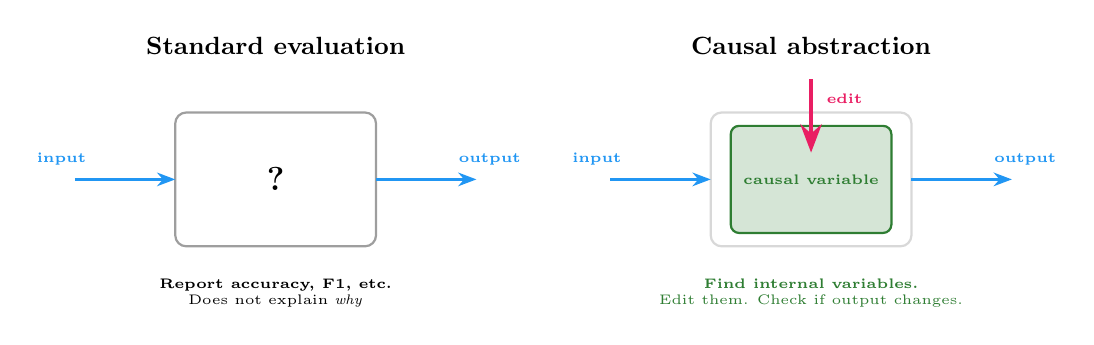
\begin{tikzpicture}[scale=0.85]
  % Left: black box
  \node[font=\small\bfseries] at (0,3.5) {Standard evaluation};
  \draw[neutral,thick,rounded corners=4pt] (-1.5,0.5) rectangle (1.5,2.5);
  \node[font=\large] at (0,1.5) {\textbf{?}};
  \draw[das,thick,-{Stealth}] (-3,1.5) -- (-1.5,1.5);
  \node[font=\tiny\bfseries,das] at (-3.2,1.8) {input};
  \draw[das,thick,-{Stealth}] (1.5,1.5) -- (3,1.5);
  \node[font=\tiny\bfseries,das] at (3.2,1.8) {output};
  \node[font=\tiny,align=center] at (0,-0.2) {\textbf{Report accuracy, F1, etc.}\\Does not explain \emph{why}};

  % Right: causal variable
  \node[font=\small\bfseries] at (8,3.5) {Causal abstraction};
  \draw[neutral!40,thick,rounded corners=4pt] (6.5,0.5) rectangle (9.5,2.5);
  \draw[das,thick,-{Stealth}] (5,1.5) -- (6.5,1.5);
  \node[font=\tiny\bfseries,das] at (4.8,1.8) {input};
  \draw[das,thick,-{Stealth}] (9.5,1.5) -- (11,1.5);
  \node[font=\tiny\bfseries,das] at (11.2,1.8) {output};

  % The causal variable inside — bigger green box, smaller text
  \fill[grass!20,rounded corners=3pt] (6.8,0.7) rectangle (9.2,2.3);
  \draw[grass,thick,rounded corners=3pt] (6.8,0.7) rectangle (9.2,2.3);
  \node[font=\tiny\bfseries,grass] at (8,1.5) {causal variable};

  % Edit arrow
  \draw[circle,ultra thick,-{Stealth}] (8,3.0) -- (8,1.9);
  \node[font=\tiny\bfseries,circle] at (8.5,2.7) {edit};

  \node[font=\tiny,grass,align=center] at (8,-0.2) {\textbf{Find internal variables.}\\Edit them. Check if output changes.};
\end{tikzpicture}

\vspace{0.3em}
{\small If editing a specific direction in the network's internal representation changes the output predictably, that direction is a \textbf{causal variable} for the behavior.}%
\footnote{\tiny Geiger et al., ``Causal Abstraction for Faithful Model Interpretation,'' 2021. \href{https://arxiv.org/abs/2301.04709}{arXiv:2301.04709}}
\end{frame}

%% --- SLIDE: Interchange intervention (original) ---
\begin{frame}{Interchange intervention analysis (IIA)}

{\small The core technique: take two inputs, swap part of their internal representations, check if the output changes accordingly.}%
\footnote{\tiny Geiger et al., ``Inducing Causal Structure for Interpretable Neural Networks,'' ICML 2022. \href{https://arxiv.org/abs/2112.00826}{arXiv:2112.00826}}

\vspace{0.5em}

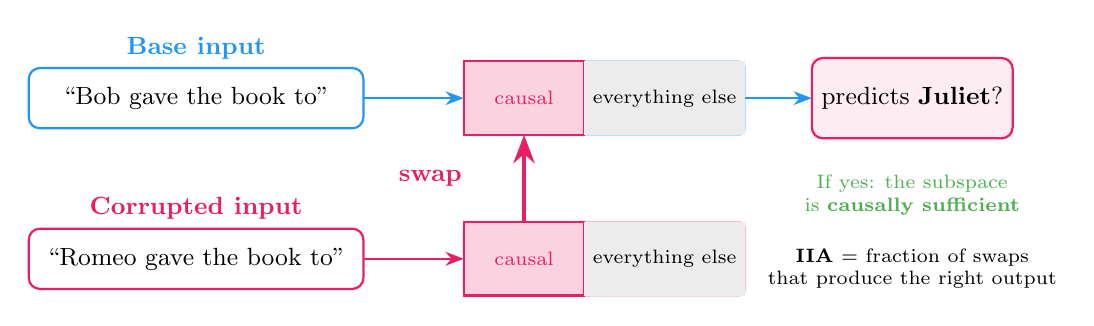
\begin{tikzpicture}[scale=0.85]
  % Base path
  \node[font=\small\bfseries,das] at (0,4.2) {Base input};
  \draw[das,thick,rounded corners=4pt] (-2.5,3.0) rectangle (2.5,3.9);
  \node[font=\small] at (0,3.45) {``Bob gave the book to''};

  % Corrupted path
  \node[font=\small\bfseries,circle] at (0,1.8) {Corrupted input};
  \draw[circle,thick,rounded corners=4pt] (-2.5,0.6) rectangle (2.5,1.5);
  \node[font=\small] at (0,1.05) {``Romeo gave the book to''};

  % Activations
  \draw[das,thick,-{Stealth}] (2.5,3.45) -- (4,3.45);
  \draw[circle,thick,-{Stealth}] (2.5,1.05) -- (4,1.05);

  % Base activation box
  \draw[das!30,thick,rounded corners=2pt] (4,2.9) rectangle (8.2,4.0);
  \fill[circle!20] (4,2.9) rectangle (5.8,4.0);
  \draw[circle,thick] (4,2.9) rectangle (5.8,4.0);
  \node[font=\scriptsize,circle] at (4.9,3.45) {causal};
  \fill[neutral!20] (5.8,2.9) rectangle (8.2,4.0);
  \node[font=\scriptsize] at (7.0,3.45) {everything else};

  % Corrupted activation box
  \draw[circle!30,thick,rounded corners=2pt] (4,0.5) rectangle (8.2,1.6);
  \fill[circle!20] (4,0.5) rectangle (5.8,1.6);
  \draw[circle,thick] (4,0.5) rectangle (5.8,1.6);
  \node[font=\scriptsize,circle] at (4.9,1.05) {causal};
  \fill[neutral!20] (5.8,0.5) rectangle (8.2,1.6);
  \node[font=\scriptsize] at (7.0,1.05) {everything else};

  % Swap arrow
  \draw[circle,ultra thick,-{Stealth}] (4.9,1.6) -- (4.9,2.9);
  \node[font=\small\bfseries,circle] at (3.5,2.25) {swap};

  % Output
  \draw[das,thick,-{Stealth}] (8.2,3.45) -- (9.2,3.45);
  \fill[circle!8] (9.2,2.85) rectangle (12.2,4.05);
  \draw[circle,thick,rounded corners=4pt] (9.2,2.85) rectangle (12.2,4.05);
  \node[font=\small,align=center] at (10.7,3.45) {predicts \textbf{Juliet}?};

  % IIA label
  \node[font=\scriptsize,pass,align=center] at (10.7,2.0) {If yes: the subspace\\is \textbf{causally sufficient}};
  \node[font=\scriptsize,align=center] at (10.7,0.9) {\textbf{IIA} = fraction of swaps\\that produce the right output};
\end{tikzpicture}
\end{frame}

\hypertarget{sec2}{}
\section{2. DAS and the Grassmannian}

%% --- SLIDE: What DAS actually does (original) ---
\begin{frame}{What DAS actually does}

\begin{columns}[T]
\begin{column}{0.55\textwidth}
{\small DAS learns a rotation matrix $Q \in \R^{d \times k}$ that identifies a $k$-dimensional subspace of the $d$-dimensional activation space.}%
\footnote{\tiny Geiger et al., ``Finding Alignments Between Interpretable Causal Variables and Distributed Neural Representations,'' 2024. \href{https://arxiv.org/abs/2303.02536}{arXiv:2303.02536}}

\vspace{0.3em}
{\small The interchange intervention projects out the base's component and replaces it with the source's:}

$$h' = h_b - QQ^\top h_b + QQ^\top h_s$$

{\small This is a \textbf{linear} operation. The subspace $QQ^\top$ is an orthogonal projection onto a \emph{flat plane} in activation space.}

\vspace{0.3em}
{\small The set of all $k$-dimensional planes in $\R^d$ is the \textbf{Grassmannian manifold} $\Gr(k,d)$.}

\vspace{0.3em}
{\small Every DAS solution is a point on $\Gr(k,d)$.}
\end{column}
\begin{column}{0.42\textwidth}
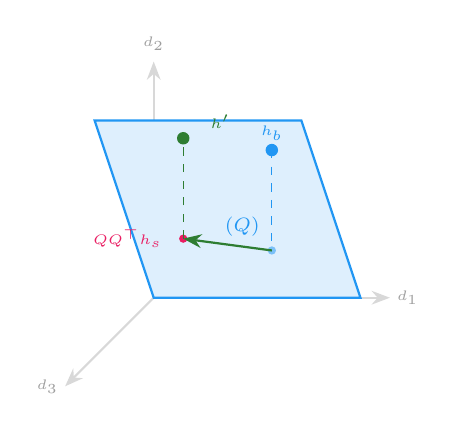
\begin{tikzpicture}[scale=0.75]
  % 3D-ish activation space
  \draw[neutral!40,thick,-{Stealth}] (0,0) -- (4,0);
  \draw[neutral!40,thick,-{Stealth}] (0,0) -- (0,4);
  \draw[neutral!40,thick,-{Stealth}] (0,0) -- (-1.5,-1.5);
  \node[font=\tiny,neutral] at (4.3,0) {$d_1$};
  \node[font=\tiny,neutral] at (0,4.3) {$d_2$};
  \node[font=\tiny,neutral] at (-1.8,-1.5) {$d_3$};

  % The subspace (a plane)
  \fill[das!15] (0,0) -- (3.5,0) -- (2.5,3) -- (-1,3) -- cycle;
  \draw[das,thick] (0,0) -- (3.5,0) -- (2.5,3) -- (-1,3) -- cycle;
  \node[font=\scriptsize,das] at (1.5,1.2) {$\Span(Q)$};

  % Base point
  \fill[das] (2,2.5) circle (3pt);
  \node[font=\tiny,das,above] at (2,2.5) {$h_b$};

  % Projection
  \draw[das,dashed] (2,2.5) -- (2,0.8);
  \fill[das!60] (2,0.8) circle (2pt);

  % Source projection
  \fill[circle] (0.5,1.0) circle (2pt);
  \node[font=\tiny,circle,left] at (0.3,1.0) {$QQ^\top h_s$};

  % Intervened point
  \draw[grass,thick,-{Stealth}] (2,0.8) -- (0.5,1.0);
  \fill[grass] (2,2.5) ++(-1.5,0.2) circle (3pt);
  \node[font=\tiny,grass,above right] at (0.8,2.7) {$h'$};
  \draw[grass,dashed] (0.5,1.0) -- (0.5,2.7);
\end{tikzpicture}

\vspace{0.3em}
\centering
{\scriptsize DAS projects onto a \textbf{flat plane}.\\What if the variable lives on a \textbf{curve}?}
\end{column}
\end{columns}
\end{frame}

%% --- SLIDE: The Grassmannian (original) ---
\begin{frame}{The Grassmannian manifold $\Gr(k,d)$}

\begin{columns}[T]
\begin{column}{0.62\textwidth}
{\small The Grassmannian $\Gr(k,d)$ is the set of all $k$-dimensional linear subspaces of $\R^d$.}

\vspace{0.3em}
{\small Think of it as a ``space of planes.'' Every DAS solution picks one plane from this space. The distance between two planes is measured by their \textbf{principal angles}:}

\vspace{-2pt}
{\small $$d_{\Gr}([Q_1],[Q_2]) = \textstyle\left(\sum_i \theta_i^2\right)^{1/2}$$}

\vspace{-6pt}
{\small When we ask ``does DAS work?'' we are really asking:}

\vspace{0.2em}
\begin{center}
\fcolorbox{grass}{grass!10}{\parbox{0.88\linewidth}{\centering\vspace{0.2em}
  {\small Does the true causal variable live on $\Gr(k,d)$?}
\vspace{0.2em}}}
\end{center}

\vspace{0.2em}
{\small If yes: DAS finds a meaningful point.\\
If no: DAS still returns a point, but it is an \textbf{artifact}.}
\end{column}
\begin{column}{0.36\textwidth}
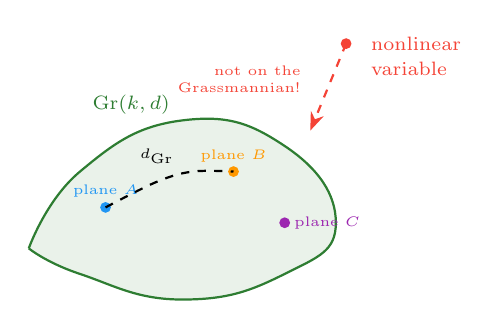
\begin{tikzpicture}[scale=0.65]
  % Grassmannian as a curved surface
  \draw[grass,thick,fill=grass!10]
    plot[smooth,tension=0.8] coordinates {(-2,0) (-1,1.5) (1,2.5) (3,2) (4,0.5) (3,-0.5) (1,-1) (-1,-0.5) (-2,0)};
  \node[font=\scriptsize\bfseries,grass] at (0,2.8) {$\Gr(k,d)$};

  % Points on it = different subspaces
  \fill[das] (-0.5,0.8) circle (3pt);
  \node[font=\tiny,das,above] at (-0.5,0.8) {plane $A$};

  \fill[stoch] (2,1.5) circle (3pt);
  \node[font=\tiny,stoch,above] at (2,1.5) {plane $B$};

  \fill[vae] (3,0.5) circle (3pt);
  \node[font=\tiny,vae,right] at (3,0.5) {plane $C$};

  % Geodesic
  \draw[black,thick,dashed]
    plot[smooth,tension=0.6] coordinates {(-0.5,0.8) (0.5,1.3) (1.2,1.5) (2,1.5)};
  \node[font=\tiny] at (0.5,1.8) {$d_{\Gr}$};

  % Off-manifold point — moved to the right
  \fill[never] (4.2,4.0) circle (3pt);
  \node[font=\scriptsize,never,right] at (4.5,4.0) {nonlinear};
  \node[font=\scriptsize,never,right] at (4.5,3.5) {variable};
  \draw[never,thick,dashed,-{Stealth}] (4.2,4.0) -- (3.5,2.3);
  \node[font=\tiny,never,left,align=right] at (3.5,3.3) {not on the\\Grassmannian!};
\end{tikzpicture}

\vspace{0.3em}
\centering
{\scriptsize A nonlinear causal variable (circle, sphere)\\does not live on $\Gr(k,d)$ at any $k$.}
\end{column}
\end{columns}
\end{frame}

\hypertarget{sec3}{}
\section{3. Why linearity matters}

%% --- SLIDE: Linear vs nonlinear causal variables ---
\begin{frame}{Linear vs.\ nonlinear causal variables}

\begin{columns}[T]
\begin{column}{0.48\textwidth}
\centering
\textbf{\textcolor{das}{Linear causal variable}}

\vspace{0.3em}
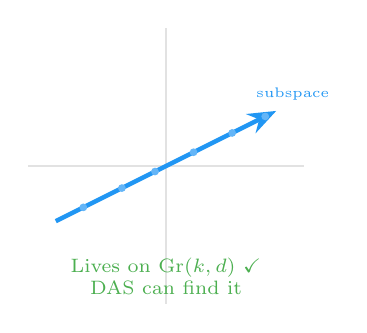
\begin{tikzpicture}[scale=0.7]
  \draw[neutral!30] (-2.5,0) -- (2.5,0);
  \draw[neutral!30] (0,-2.5) -- (0,2.5);

  % Linear subspace
  \draw[das,ultra thick,-{Stealth}] (-2,-1) -- (2,1);
  \node[font=\tiny,das] at (2.3,1.3) {subspace};

  % Points projected onto line
  \foreach \x/\y in {-1.5/-0.75, -0.8/-0.4, -0.2/-0.1, 0.5/0.25, 1.2/0.6, 1.8/0.9} {
    \fill[das!70] (\x,\y) circle (2pt);
  }

  \node[font=\scriptsize,pass,align=center] at (0,-2) {Lives on $\Gr(k,d)$ \checkmark\\DAS can find it};
\end{tikzpicture}

\vspace{0.3em}
{\small Examples: IOI indirect object (partially), multiplication mod $p$ after grokking}
\end{column}
\begin{column}{0.48\textwidth}
\centering
\textbf{\textcolor{circle}{Nonlinear causal variable}}

\vspace{0.3em}
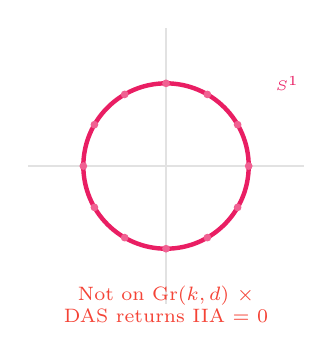
\begin{tikzpicture}[scale=0.7]
  \draw[neutral!30] (-2.5,0) -- (2.5,0);
  \draw[neutral!30] (0,-2.5) -- (0,2.5);

  % Circle
  \draw[circle,ultra thick] (0,0) circle (1.5);

  % Points on circle
  \foreach \a in {0,30,...,330} {
    \fill[circle!70] ({1.5*cos(\a)},{1.5*sin(\a)}) circle (2pt);
  }
  \node[font=\tiny,circle] at (2.2,1.5) {$S^1$};

  \node[font=\scriptsize,fail,align=center] at (0,-2.5) {Not on $\Gr(k,d)$ $\times$\\DAS returns IIA = 0};
\end{tikzpicture}

\vspace{0.3em}
{\small Examples: addition mod $p$ after grokking (Fourier representation encodes numbers on a circle)}
\end{column}
\end{columns}
\end{frame}

%% --- SLIDE: The central question ---
\begin{frame}{The central question}

\begin{center}
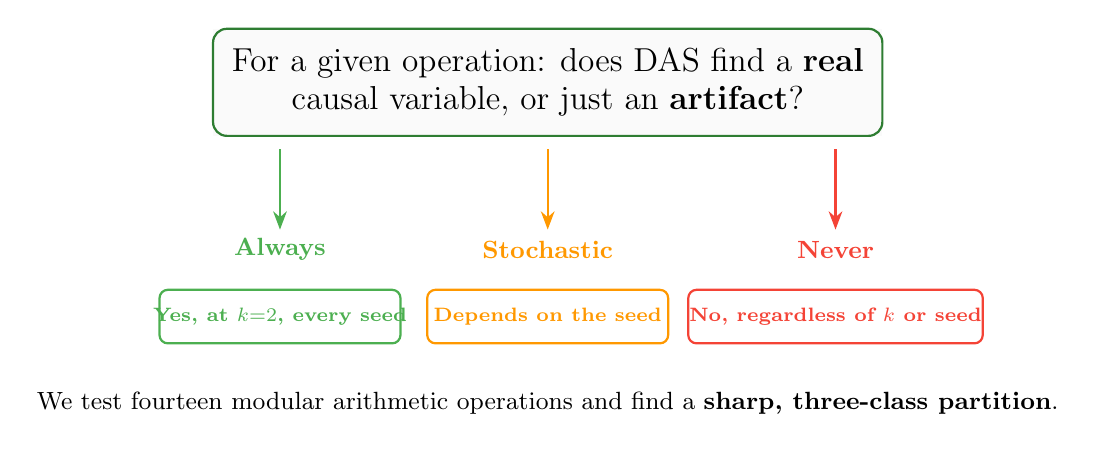
\begin{tikzpicture}[scale=0.85]
  % Question box
  \fill[bg] (-5,-0.8) rectangle (5,0.8);
  \draw[grass,thick,rounded corners=5pt] (-5,-0.8) rectangle (5,0.8);
  \node[font=\large,align=center] at (0,0) {For a given operation: does DAS find a \textbf{real}\\causal variable, or just an \textbf{artifact}?};

  % Three possibilities
  \node[font=\small\bfseries,always] at (-4,-2.5) {Always};
  \draw[always,thick,rounded corners=3pt] (-5.8,-3.1) rectangle (-2.2,-3.9);
  \node[font=\scriptsize,always,align=center] at (-4,-3.5) {\textbf{Yes, at $k{=}2$, every seed}};

  \node[font=\small\bfseries,stoch] at (0,-2.5) {Stochastic};
  \draw[stoch,thick,rounded corners=3pt] (-1.8,-3.1) rectangle (1.8,-3.9);
  \node[font=\scriptsize,stoch,align=center] at (0,-3.5) {\textbf{Depends on the seed}};

  \node[font=\small\bfseries,never] at (4.3,-2.5) {Never};
  \draw[never,thick,rounded corners=3pt] (2.1,-3.1) rectangle (6.5,-3.9);
  \node[font=\scriptsize,never,align=center] at (4.3,-3.5) {\textbf{No, regardless of $k$ or seed}};

  % Arrows
  \draw[always,thick,-{Stealth}] (-4,-1.0) -- (-4,-2.2);
  \draw[stoch,thick,-{Stealth}] (0,-1.0) -- (0,-2.2);
  \draw[never,thick,-{Stealth}] (4.3,-1.0) -- (4.3,-2.2);

  % Bottom line
  \node[font=\small,align=center] at (0,-4.8) {We test fourteen modular arithmetic operations and find a \textbf{sharp, three-class partition}.};
\end{tikzpicture}
\end{center}
\end{frame}

%% --- SLIDE: Why subspaces matter for circuits ---
\begin{frame}{Why subspaces matter for circuits}

\begin{columns}[T]
\begin{column}{0.48\textwidth}
{\small Mechanistic interpretability asks two questions about neural network circuits:}

\vspace{0.5em}
\textbf{\textcolor{das}{Q1: Which components?}}\\[0.2em]
{\small Which attention heads and MLPs matter for a behavior? Which edges carry the signal?}

\vspace{0.3em}
{\footnotesize Methods: activation patching, attribution patching, EAP.}

\vspace{0.5em}
\textbf{\textcolor{vae}{Q2: What do they communicate?}}\\[0.2em]
{\small When two components are connected, \emph{what} flows between them? Which subspaces of the residual stream carry the signal?}

\vspace{0.3em}
{\footnotesize Methods: DAS, probing, SAEs.}
\end{column}
\begin{column}{0.48\textwidth}
\vspace{0.5em}
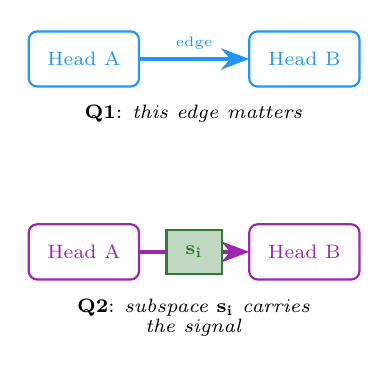
\begin{tikzpicture}[scale=0.7]
  % Edge (Q1)
  \draw[das,thick,rounded corners=3pt] (-1,4.5) rectangle (1,5.5);
  \node[font=\scriptsize,das] at (0,5.0) {Head A};
  \draw[das,thick,rounded corners=3pt] (3,4.5) rectangle (5,5.5);
  \node[font=\scriptsize,das] at (4,5.0) {Head B};
  \draw[das,ultra thick,-{Stealth}] (1,5.0) -- (3,5.0);
  \node[font=\tiny,das,above] at (2,5.0) {edge};
  \node[font=\scriptsize] at (2,4.0) {\textbf{Q1}: \emph{this edge matters}};

  % Subspace (Q2)
  \draw[vae,thick,rounded corners=3pt] (-1,1.0) rectangle (1,2.0);
  \node[font=\scriptsize,vae] at (0,1.5) {Head A};
  \draw[vae,thick,rounded corners=3pt] (3,1.0) rectangle (5,2.0);
  \node[font=\scriptsize,vae] at (4,1.5) {Head B};
  \draw[vae,ultra thick,-{Stealth}] (1,1.5) -- (3,1.5);
  \fill[grass!30] (1.5,1.1) rectangle (2.5,1.9);
  \draw[grass,thick] (1.5,1.1) rectangle (2.5,1.9);
  \node[font=\scriptsize,grass] at (2,1.5) {$\mathbf{s_i}$};
  \node[font=\scriptsize,align=center] at (2,0.3) {\textbf{Q2}: \emph{subspace $\mathbf{s_i}$ carries}\\[-0.1em]\emph{the signal}};
\end{tikzpicture}

\vspace{0.3em}
\fcolorbox{grass}{grass!10}{\parbox{0.9\linewidth}{\centering\vspace{0.2em}
  {\small Our work: whether Q2 has a \textbf{linear} answer depends on the operation.}
\vspace{0.2em}}}
\end{column}
\end{columns}

\end{frame}


%% PART 4: THE FIX
%% ============================================================

\begin{frame}[plain]
\vfill
\begin{center}
  \setlength{\fboxrule}{2.5pt}%
  \fcolorbox{black}{white}{\parbox{0.7\textwidth}{\centering\vspace{0.8em}
    {\Large\bfseries Part 4}\hypertarget{part4}{}\\[0.5em]
    {\large The fix: structured VAE and cross-task transfer}
  \vspace{0.8em}}}
\end{center}
\vfill
\end{frame}


\hypertarget{sec10}{}
\section{10. Structured VAE}

%% --- SLIDE: The structured VAE idea ---
\begin{frame}{Structured VAE for nonlinear causal variables}

\begin{columns}[T]
\begin{column}{0.55\textwidth}
{\small The structured VAE partitions the latent space into:}
\begin{itemize}
  \item {\small $z_\text{causal}$: supervised with the operation's label}
  \item {\small $z_\text{nuisance}$: unsupervised, absorbs everything else}
\end{itemize}

\vspace{0.3em}
{\small The loss combines three terms:}
$$\mathcal{L} = \underbrace{-\mathbb{E}_q[\log p(x \mid y, z)]}_{\text{reconstruction}} + \beta \underbrace{D_\text{KL}}_{\text{regularization}} + \alpha \underbrace{\mathcal{L}_\text{CE}}_{\text{supervision}}$$

\vspace{0.3em}
{\small The ELBO prevents the lookup-table failure:}
\begin{enumerate}
  \item {\small Reconstruction forces faithful decoding}
  \item {\small KL prevents latent collapse}
  \item {\small Causal/nuisance split preserves base info}
\end{enumerate}
\end{column}
\begin{column}{0.42\textwidth}
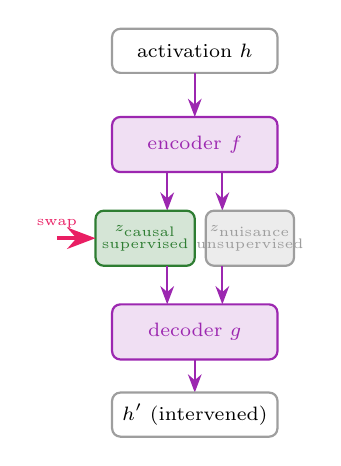
\begin{tikzpicture}[scale=0.7]
  % Input
  \draw[neutral,thick,rounded corners=3pt] (-1.5,5.0) rectangle (1.5,5.8);
  \node[font=\scriptsize] at (0,5.4) {activation $h$};

  % Encoder
  \draw[vae,thick,-{Stealth}] (0,5.0) -- (0,4.2);
  \draw[vae,thick,rounded corners=3pt,fill=vae!15] (-1.5,3.2) rectangle (1.5,4.2);
  \node[font=\scriptsize,vae] at (0,3.7) {encoder $f$};

  % Split
  \draw[vae,thick,-{Stealth}] (-0.5,3.2) -- (-0.5,2.5);
  \draw[vae,thick,-{Stealth}] (0.5,3.2) -- (0.5,2.5);

  % Causal latent
  \fill[grass!20,rounded corners=3pt] (-1.8,1.5) rectangle (0,2.5);
  \draw[grass,thick,rounded corners=3pt] (-1.8,1.5) rectangle (0,2.5);
  \node[font=\tiny,grass,align=center] at (-0.9,2.0) {$z_\text{causal}$\\{\tiny supervised}};

  % Nuisance latent
  \fill[neutral!20,rounded corners=3pt] (0.2,1.5) rectangle (1.8,2.5);
  \draw[neutral,thick,rounded corners=3pt] (0.2,1.5) rectangle (1.8,2.5);
  \node[font=\tiny,neutral,align=center] at (1.0,2.0) {$z_\text{nuisance}$\\{\tiny unsupervised}};

  % Swap arrow
  \draw[circle,ultra thick,-{Stealth}] (-2.5,2.0) -- (-1.8,2.0);
  \node[font=\tiny,circle,above] at (-2.5,2.0) {swap};

  % Decoder
  \draw[vae,thick,-{Stealth}] (-0.5,1.5) -- (-0.5,0.8);
  \draw[vae,thick,-{Stealth}] (0.5,1.5) -- (0.5,0.8);
  \draw[vae,thick,rounded corners=3pt,fill=vae!15] (-1.5,-0.2) rectangle (1.5,0.8);
  \node[font=\scriptsize,vae] at (0,0.3) {decoder $g$};

  % Output
  \draw[vae,thick,-{Stealth}] (0,-0.2) -- (0,-0.8);
  \draw[neutral,thick,rounded corners=3pt] (-1.5,-1.6) rectangle (1.5,-0.8);
  \node[font=\scriptsize] at (0,-1.2) {$h'$ (intervened)};
\end{tikzpicture}
\end{column}
\end{columns}
\end{frame}

%% --- SLIDE: Why VAE is not vacuous ---
\begin{frame}{Why the VAE is not vacuous: three constraints}
\vspace{-0.5em}

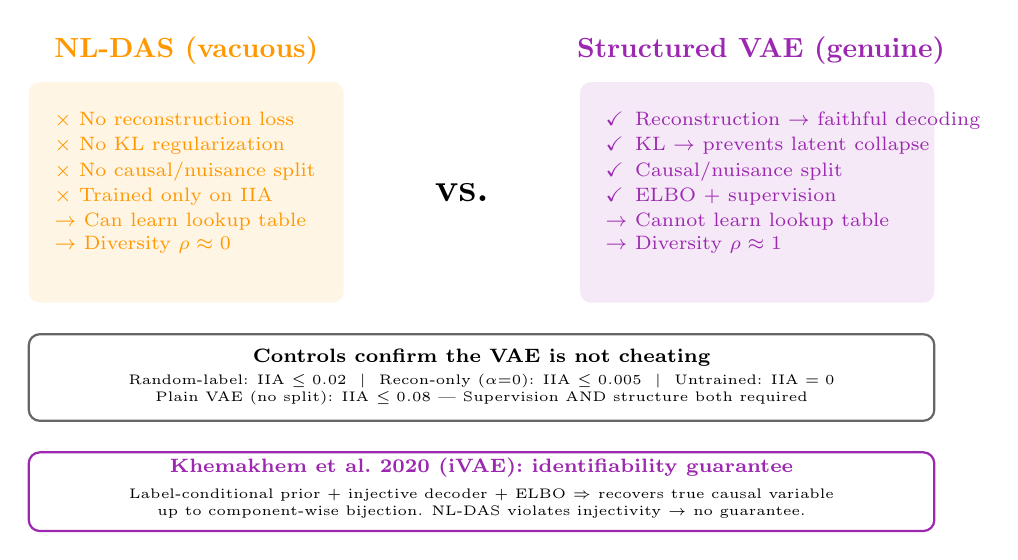
\begin{tikzpicture}[scale=1.0, transform shape]
  % NL-DAS column
  \node[font=\normalsize\bfseries,nldas] at (-3.5,4.2) {NL-DAS (vacuous)};

  \fill[nldas!10,rounded corners=4pt] (-5.5,1.0) rectangle (-1.5,3.8);
  \node[font=\scriptsize,nldas,align=left,anchor=north west] at (-5.3,3.55) {%
    $\times$ No reconstruction loss\\[0.15em]
    $\times$ No KL regularization\\[0.15em]
    $\times$ No causal/nuisance split\\[0.15em]
    $\times$ Trained only on IIA\\[0.15em]
    $\to$ Can learn lookup table\\
    $\to$ Diversity $\rho \approx 0$};

  % Arrow
  \node[font=\Large\bfseries] at (0,2.4) {vs.};

  % VAE column
  \node[font=\normalsize\bfseries,vae] at (3.8,4.2) {Structured VAE (genuine)};

  \fill[vae!10,rounded corners=4pt] (1.5,1.0) rectangle (6.0,3.8);
  \node[font=\scriptsize,vae,align=left,anchor=north west] at (1.7,3.55) {%
    \checkmark\, Reconstruction $\to$ faithful decoding\\[0.15em]
    \checkmark\, KL $\to$ prevents latent collapse\\[0.15em]
    \checkmark\, Causal/nuisance split\\[0.15em]
    \checkmark\, ELBO + supervision\\[0.15em]
    $\to$ Cannot learn lookup table\\
    $\to$ Diversity $\rho \approx 1$};

  % Controls
  \draw[black!60,thick,rounded corners=4pt] (-5.5,-0.5) rectangle (6.0,0.6);
  \node[font=\scriptsize\bfseries] at (0.25,0.3) {Controls confirm the VAE is not cheating};
  \node[font=\tiny,align=center] at (0.25,-0.1) {Random-label: IIA $\leq 0.02$ ~$|$~ Recon-only ($\alpha{=}0$): IIA $\leq 0.005$ ~$|$~ Untrained: IIA $= 0$\\
  Plain VAE (no split): IIA $\leq 0.08$ --- Supervision AND structure both required};

  % Identifiability takeaway
  \draw[vae,thick,rounded corners=4pt] (-5.5,-1.9) rectangle (6.0,-0.9);
  \node[font=\scriptsize\bfseries,vae] at (0.25,-1.1) {Khemakhem et al.\ 2020 (iVAE): identifiability guarantee};
  \node[font=\tiny,align=center] at (0.25,-1.55) {Label-conditional prior + injective decoder + ELBO $\Rightarrow$ recovers true causal variable\\
  up to component-wise bijection. NL-DAS violates injectivity $\to$ no guarantee.};
\end{tikzpicture}
\end{frame}

%% --- SLIDE: VAE matches DAS where DAS works ---
\begin{frame}{VAE matches DAS where DAS works, extends where it fails}

\begin{columns}[T]
\begin{column}{0.48\textwidth}
{\small \textbf{Always Grassmannian operations:}\\VAE reduces to an effective rotation.}

\vspace{0.3em}
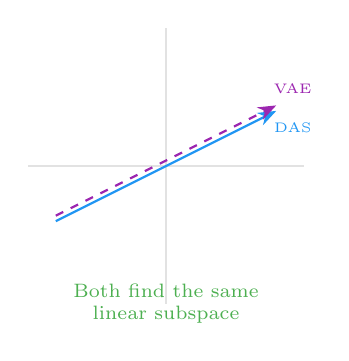
\begin{tikzpicture}[scale=0.7]
  % DAS and VAE agree
  \draw[neutral!30] (-2.5,0) -- (2.5,0);
  \draw[neutral!30] (0,-2.5) -- (0,2.5);

  % Linear subspace
  \draw[das,thick,-{Stealth}] (-2,-1) -- (2,1);
  \draw[vae,thick,dashed,-{Stealth}] (-2,-0.9) -- (2,1.1);

  \node[font=\tiny,das] at (2.3,0.7) {DAS};
  \node[font=\tiny,vae] at (2.3,1.4) {VAE};

  \node[font=\scriptsize,pass,align=center] at (0,-2.5) {Both find the same\\linear subspace};
\end{tikzpicture}
\end{column}
\begin{column}{0.48\textwidth}
{\small \textbf{Never Grassmannian operations:}\\VAE's nonlinear encoder captures curved structure.}

\vspace{0.3em}
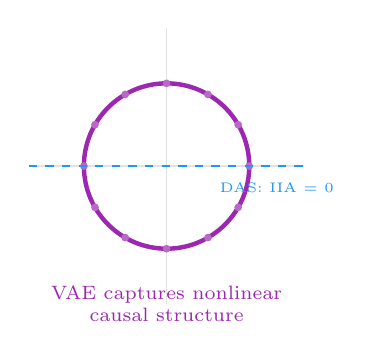
\begin{tikzpicture}[scale=0.7]
  \draw[neutral!30] (-2.5,0) -- (2.5,0);
  \draw[neutral!30] (0,-2.5) -- (0,2.5);

  % Circle
  \draw[vae,ultra thick] (0,0) circle (1.5);
  \foreach \a in {0,30,...,330} {
    \fill[vae!70] ({1.5*cos(\a)},{1.5*sin(\a)}) circle (2pt);
  }

  % DAS fails
  \draw[das,thick,dashed] (-2.5,0) -- (2.5,0);
  \node[font=\tiny,das] at (2.0,-0.4) {DAS: IIA = 0};

  \node[font=\scriptsize,vae,align=center] at (0,-2.5) {VAE captures nonlinear\\causal structure};
\end{tikzpicture}
\end{column}
\end{columns}

\vspace{0.5em}
\centering
{\small For grokked addition and multiplication, both DAS and VAE achieve IIA = 1.000 and equivariance $>99\%$.\\The VAE is a \textbf{strict generalization} of DAS: when the variable is linear, VAE = DAS.}
\end{frame}

\hypertarget{sec10b}{}
\section{10b. Structured pi-SAE: sparse nonlinear causal discovery}

%% --- SLIDE: From VAE to Structured pi-SAE ---
\begin{frame}{From pi-VAE to Structured pi-SAE: sparsity + structure}

\begin{columns}[T]
\begin{column}{0.48\textwidth}
\textbf{pi-VAE} {\small (Zhou \& Wei, 2020)}\\[0.3em]
{\small Label-conditional prior:}
\vspace{-0.2em}
\[ p(z \mid y) = \mathcal{N}\!\bigl(\mu(y),\, \sigma^2(y)\bigr) \]
\vspace{-0.5em}
{\small Each label gets its own mean and variance. Forces the latent space to organize by label.}

\vspace{0.5em}
{\small Published method. Works well on IOI.\\[0.2em]
But on grokked modular arithmetic:\\
IIA $= 0$ across all $k$.}
\end{column}
\begin{column}{0.48\textwidth}
\textbf{Structured pi-SAE} {\small \textcolor{vae}{(ours)}}\\[0.3em]
{\small pi-VAE + \textbf{causal/nuisance split} + \textbf{L1 sparsity}:}
\vspace{-0.2em}
\[ \mathcal{L} = \mathcal{L}_\text{pi-VAE} + \lambda \|z_c\|_1, \quad z = (z_c, z_n) \]
\vspace{-0.5em}
{\small Explicit causal/nuisance partition forces the model to separate task-relevant from task-irrelevant variation.}

\vspace{0.3em}
{\small L1 sparsity on $z_c$ prevents memorization --- the encoder can't just copy the input.}
\end{column}
\end{columns}

\vspace{0.5em}
\centering
\fcolorbox{vae}{vae!8}{\parbox{0.85\textwidth}{\centering\vspace{0.1em}
{\small \textbf{Two modifications} over pi-VAE: (1) causal/nuisance split in the latent space, (2) L1 sparsity on causal dimensions. Neither alone suffices.}
\vspace{0.1em}}}
\end{frame}

%% --- SLIDE: pi-SAE vs pi-VAE results ---
\begin{frame}{Structured pi-SAE vs.\ pi-VAE: results}

\begin{columns}[T]
\begin{column}{0.48\textwidth}
{\small IIA at $k{=}2$. Controls $\leq 0.02$.}

\vspace{0.5em}
\centering
{\small
\begin{tabular}{@{}lcc@{}}
\toprule
& \textbf{pi-VAE} & \textbf{Str.\ pi-SAE} \\
\midrule
Addition & 0.000 & \textcolor{always}{1.000} \\
Multiplication & 0.000 & \textcolor{always}{1.000} \\
Quartic sum & 0.000 & \textcolor{always}{1.000} \\
IOI (GPT-2) & 0.945 & \textcolor{always}{0.980} \\
\midrule
Mixed product & 0.010 & 0.040 \\
Squaring & 0.000 & 0.000 \\
\bottomrule
\end{tabular}}

\vspace{0.3em}
\flushleft
{\scriptsize Non-grokked operations correctly return $\approx 0$.}
\end{column}
\begin{column}{0.48\textwidth}
{\small \textbf{What changed:}}

\vspace{0.3em}
{\small pi-VAE gets IIA $= 0$ on \textit{every} grokking task. The structured prior alone is not enough --- the latent space collapses without the sparsity constraint.}

\vspace{0.5em}
{\small Adding the causal/nuisance split + L1:}
\begin{itemize}\setlength{\itemsep}{2pt}
  \item {\small All grokked operations $\to$ IIA $= 1.0$}
  \item {\small IOI $\to$ IIA $= 0.98$}
  \item {\small Non-grokked $\to$ IIA $\approx 0$ (correct rejection)}
\end{itemize}

\vspace{0.5em}
\fcolorbox{always}{always!8}{\parbox{0.9\linewidth}{\centering\vspace{0.1em}
{\small Sparsity is the missing ingredient.}
\vspace{0.1em}}}
\end{column}
\end{columns}
\end{frame}

%% --- SLIDE: Intrinsic dimension ---
\begin{frame}{Intrinsic dimension: $k{=}1$ reveals the true structure}
\vspace{-0.3em}

\begin{columns}[T]
\begin{column}{0.50\textwidth}
{\small A circle is \textbf{1-dimensional} --- one angle $\theta$.
Linear DAS needs $k{=}2$: embeds as $(\cos\theta, \sin\theta)$.
A nonlinear method learns $z = \theta$ directly.}

\vspace{0.3em}
{\small \textbf{Structured pi-SAE at $k{=}1$}:}

\vspace{0.2em}
{\scriptsize\setlength{\tabcolsep}{3pt}
\begin{tabular}{@{}lccc@{}}
\toprule
& \textbf{DAS} & \textbf{NL-DAS} & \textbf{Str.\ pi-SAE} \\
\midrule
Addition & 0.006 & 0.194 & \textbf{\textcolor{always}{0.917}} \\
Multiplication & 0.022 & 0.217 & 0.011 \\
Quartic sum & 0.011 & 0.244 & 0.106 \\
IOI & 0.185 & 1.000 & \textbf{\textcolor{always}{0.988}} \\
\bottomrule
\end{tabular}}

\vspace{0.2em}
{\scriptsize Addition's circle admits a smooth 1D parameterization. Multiplication's discrete-log circle does not.}
\end{column}
\begin{column}{0.46\textwidth}
\centering
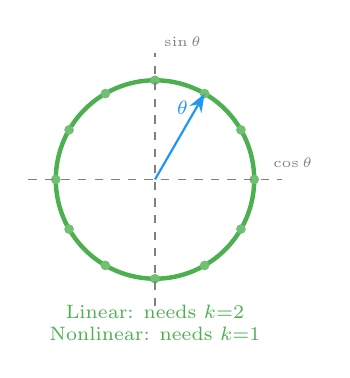
\begin{tikzpicture}[scale=0.7]
  \draw[always,ultra thick] (0,0) circle (1.8);

  \foreach \a in {0, 30, 60, 90, 120, 150, 180, 210, 240, 270, 300, 330} {
    \fill[always!80] ({1.8*cos(\a)},{1.8*sin(\a)}) circle (2.5pt);
  }

  \draw[das,thick,-{Stealth}] (0,0) -- ({1.8*cos(60)},{1.8*sin(60)});
  \node[font=\scriptsize,das] at (0.5,1.3) {$\theta$};

  \draw[gray,thin,dashed] (-2.3,0) -- (2.3,0);
  \draw[gray,thin,dashed] (0,-2.3) -- (0,2.3);
  \node[font=\tiny,gray] at (2.5,0.3) {$\cos\theta$};
  \node[font=\tiny,gray] at (0.5,2.5) {$\sin\theta$};

  \node[font=\scriptsize,always,align=center] at (0,-2.6) {Linear: needs $k{=}2$\\Nonlinear: needs $k{=}1$};
\end{tikzpicture}

\vspace{0.3em}
\fcolorbox{always}{always!8}{\parbox{0.9\linewidth}{\centering\vspace{0.1em}
  {\small Linear DAS \textbf{overestimates}\\intrinsic dimension.}
\vspace{0.1em}}}
\end{column}
\end{columns}
\end{frame}

%% --- SLIDE: Full results table ---
\begin{frame}{Structured pi-SAE results across all operations}
\vspace{-0.5em}
\centering
{\scriptsize\setlength{\tabcolsep}{2.5pt}
\begin{tabular}{@{}lcccccccc@{}}
\toprule
& & & \multicolumn{3}{c}{\textbf{IIA at $k{=}2$}} & \multicolumn{3}{c}{\textbf{IIA at $k{=}1$}} \\
\cmidrule(lr){4-6} \cmidrule(lr){7-9}
\textbf{Operation} & \textbf{Grok} & \textbf{Acc} & \textbf{DAS} & \textbf{NL-DAS} & \textbf{Str.\ pi-SAE} & \textbf{DAS} & \textbf{NL-DAS} & \textbf{Str.\ pi-SAE} \\
\midrule
Addition & \textcolor{always}{\checkmark} & 1.00 & 0.06 & 0.49 & \textbf{\textcolor{always}{1.00}} & 0.01 & 0.19 & \textbf{\textcolor{always}{0.92}} \\
Multiplication & \textcolor{always}{\checkmark} & 1.00 & 0.08 & 0.72 & \textbf{\textcolor{always}{1.00}} & 0.02 & 0.22 & 0.01 \\
Quartic sum & \textcolor{always}{\checkmark} & 1.00 & 0.03 & 0.79 & \textbf{\textcolor{always}{1.00}} & 0.01 & 0.24 & 0.11 \\
IOI (GPT-2) & --- & --- & 0.30 & \textcolor{never}{1.00} & \textbf{\textcolor{always}{0.98}} & 0.19 & \textcolor{never}{1.00} & \textbf{\textcolor{always}{0.99}} \\
\midrule
Mixed product & \textcolor{never}{$\times$} & 0.15 & 0.02 & \textcolor{never}{0.60} & 0.04 & 0.01 & 0.21 & 0.02 \\
Sym.\ power & \textcolor{never}{$\times$} & 0.21 & 0.02 & \textcolor{never}{0.63} & 0.02 & 0.01 & 0.26 & 0.02 \\
Dbl.\ add mult & \textcolor{never}{$\times$} & 0.10 & 0.00 & \textcolor{never}{0.77} & 0.02 & 0.00 & 0.22 & 0.02 \\
Squaring & \textcolor{never}{$\times$} & 0.01 & 0.00 & 0.01 & 0.00 & 0.00 & 0.01 & 0.00 \\
\bottomrule
\end{tabular}}

\vspace{0.4em}
{\scriptsize \textcolor{always}{Green bold}: genuine causal variable found. \textcolor{never}{Red}: NL-DAS vacuity --- high IIA despite no learned structure.}

\vspace{0.2em}
{\small Str.\ pi-SAE: IIA $= 1.0$ on all grokked, $\approx 0$ on all non-grokked. NL-DAS: 0.6--0.8 on non-grokked --- \textbf{false positives}.}
\end{frame}

%% --- SLIDE: The 2x2 ablation ---
\begin{frame}{Ablation: both sparsity and structure are required}
\vspace{-0.3em}
\centering

{\small IIA at $k{=}2$: \{structured, plain prior\} $\times$ \{VAE, SAE\}.}

\vspace{0.3em}
{\scriptsize\setlength{\tabcolsep}{3.5pt}
\begin{tabular}{@{}l|cc|cc@{}}
\toprule
& \multicolumn{2}{c|}{\textbf{Plain prior} $\mathcal{N}(0,I)$} & \multicolumn{2}{c}{\textbf{Structured prior} $p(z|y)$} \\
\textbf{Operation} & VAE & SAE & pi-VAE & \textbf{Str.\ pi-SAE} \\
\midrule
Addition & 0.02 & \textcolor{always}{1.00} & 0.00 & \textbf{\textcolor{always}{1.00}} \\
Multiplication & 0.00 & 0.72 & 0.00 & \textbf{\textcolor{always}{1.00}} \\
Quartic sum & 0.02 & 0.32 & 0.00 & \textbf{\textcolor{always}{1.00}} \\
IOI & 0.56 & 0.83 & \textcolor{always}{0.95} & \textbf{\textcolor{always}{0.98}} \\
\midrule
Mixed product & 0.03 & 0.01 & 0.01 & 0.04 \\
Squaring & 0.00 & 0.00 & 0.00 & 0.00 \\
\bottomrule
\end{tabular}}

\vspace{0.8em}
\begin{columns}[T]
\begin{column}{0.48\textwidth}
\fcolorbox{never}{never!8}{\parbox{0.9\linewidth}{\centering\vspace{0.1em}
  {\scriptsize \textbf{Plain SAE} works on addition but degrades on multiplication and quartic sum.}
\vspace{0.1em}}}
\end{column}
\begin{column}{0.48\textwidth}
\fcolorbox{always}{always!8}{\parbox{0.9\linewidth}{\centering\vspace{0.1em}
  {\scriptsize \textbf{Structured pi-SAE} is uniformly best. Prior + sparsity = robust across all tasks.}
\vspace{0.1em}}}
\end{column}
\end{columns}

\vspace{0.3em}
\centering
{\scriptsize Neither component alone suffices: pi-VAE (no sparsity, no split) $= 0$; SAE (no structured prior) is inconsistent.}
\end{frame}

%% --- SLIDE: NL-DAS vacuity exposed ---
\begin{frame}{Structured pi-SAE exposes NL-DAS vacuity}
\vspace{-0.3em}

\begin{columns}[T]
\begin{column}{0.48\textwidth}
{\small\textbf{The problem:} NL-DAS achieves IIA $= 0.6$--$0.8$ on operations that \textbf{never learned} the task (acc $< 20\%$). These are false positives --- the encoder learned a lookup table.}

\vspace{0.3em}
{\small\textbf{Structured pi-SAE correctly rejects:} IIA $\leq 0.04$ on the same operations. Reconstruction prevents hallucination.}

\vspace{0.3em}
{\scriptsize Reconstruction MSE confirms:}\\[0.1em]
{\scriptsize\setlength{\tabcolsep}{3pt}
\begin{tabular}{@{}lcc@{}}
& \textbf{Grokked} & \textbf{Not grokked} \\
\midrule
Recon MSE & 0.6--1.2 & 11--24 \\
Classifier acc & 1.00 & 0.06--0.63 \\
\end{tabular}}

\vspace{0.1em}
{\scriptsize High MSE + low acc = no structure to recover.}
\end{column}
\begin{column}{0.48\textwidth}
\centering
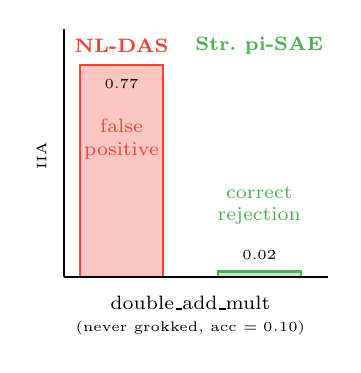
\begin{tikzpicture}[scale=0.7]
  \fill[never!30] (0,0) rectangle (1.5,3.85);
  \draw[never,thick] (0,0) rectangle (1.5,3.85);
  \node[font=\scriptsize\bfseries,never] at (0.75,4.2) {NL-DAS};
  \node[font=\tiny] at (0.75,3.5) {0.77};

  \fill[always!30] (2.5,0) rectangle (4.0,0.1);
  \draw[always,thick] (2.5,0) rectangle (4.0,0.1);
  \node[font=\scriptsize\bfseries,always] at (3.25,4.2) {Str.\ pi-SAE};
  \node[font=\tiny] at (3.25,0.4) {0.02};

  \draw[thick] (-0.3,0) -- (4.5,0);
  \draw[thick] (-0.3,0) -- (-0.3,4.5);
  \node[font=\tiny,rotate=90] at (-0.7,2.2) {IIA};
  \node[font=\scriptsize,align=center] at (2.0,-0.7) {double\_add\_mult\\{\tiny(never grokked, acc $= 0.10$)}};

  \node[font=\scriptsize,never,align=center] at (0.75,2.5) {false\\positive};
  \node[font=\scriptsize,always,align=center] at (3.25,1.3) {correct\\rejection};
\end{tikzpicture}
\end{column}
\end{columns}

\vspace{0.3em}
\begin{columns}[T]
\begin{column}{0.48\textwidth}
\end{column}
\begin{column}{0.50\textwidth}
\fcolorbox{vae}{vae!8}{\parbox{0.95\linewidth}{\vspace{0.3em}
\centering
{\small \textbf{IOI (GPT-2):}}\\[0.4em]
{\small NL-DAS: IIA $= 1.0$, $\rho \approx 0$}\\
{\small \textcolor{never}{(lookup table)}}\\[0.3em]
{\small Str.\ pi-SAE: IIA $= 0.98$, $\rho \approx 0.91$}\\
{\small \textcolor{always}{(genuine causal variable)}}
\vspace{0.3em}}}
\end{column}
\end{columns}
\end{frame}

%% --- SLIDE: CRT composite modulus ---
\begin{frame}{CRT composite modulus: the first task needing $k{>}1$}
\begin{columns}[T]
\begin{column}{0.48\textwidth}
\textbf{Chinese Remainder Theorem.}\\[0.3em]
For composite modulus $n = p \times q$:
\[ \mathbb{Z}/n\mathbb{Z} \;\cong\; \mathbb{Z}/p\mathbb{Z} \times \mathbb{Z}/q\mathbb{Z} \]
The model learns \textbf{two independent circles} ---
one mod $p$, one mod $q$.\\[0.3em]

{\small
Intrinsic dimension = \textbf{2} (two angles $\theta_p, \theta_q$).\\
Linear DAS needs $k \geq 4$ ($\cos/\sin$ for each).\\
Structured pi-SAE captures both at $k{=}2$.}\\[0.5em]

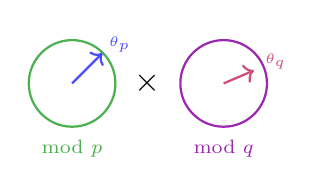
\begin{tikzpicture}[scale=0.55]
  \draw[always,thick] (0,0) circle (1.0);
  \node[font=\scriptsize,always] at (0,-1.5) {mod $p$};
  \draw[->,thick,blue!70] (0,0) -- (0.7,0.7);
  \node[font=\tiny,blue!70] at (1.1,0.9) {$\theta_p$};
  \draw[vae,thick] (3.5,0) circle (1.0);
  \node[font=\scriptsize,vae] at (3.5,-1.5) {mod $q$};
  \draw[->,thick,purple!70] (3.5,0) -- (4.2,0.3);
  \node[font=\tiny,purple!70] at (4.7,0.5) {$\theta_q$};
  \node[font=\large] at (1.75,0) {$\times$};
\end{tikzpicture}
\end{column}
\begin{column}{0.52\textwidth}
{\scriptsize
\begin{tabular}{@{}lcrrrl@{}}
\toprule
\textbf{Task} & $k$ & \textbf{DAS} & \textbf{NL-D} & \textbf{Str.\ pi-SAE} & \\
\midrule
add 113 & 1 & 0.01 & 0.19 & \textcolor{always}{\textbf{0.92}} & {\color{always}\checkmark} \\
(prime) & 2 & 0.06 & 0.49 & \textcolor{always}{\textbf{1.00}} & \\[0.2em]
add mod 77 & 1 & 0.02 & 0.19 & 0.06 & {\color{always}\checkmark} \\
($7 \times 11$) & 2 & 0.07 & 0.59 & \textcolor{always}{\textbf{0.99}} & \\[0.2em]
add mod 91 & 1 & 0.02 & 0.24 & 0.00 & {\color{always}\checkmark} \\
($7 \times 13$) & 2 & 0.16 & 0.70 & \textcolor{always}{\textbf{0.98}} & \\[0.2em]
add mod 35 & 2 & 0.08 & \textcolor{never}{\textbf{0.51}} & 0.21 & {\color{never}$\times$} \\
($5 \times 7$) & 4 & 0.21 & \textcolor{never}{\textbf{0.95}} & 0.21 & \\
\bottomrule
\end{tabular}
}\\[0.3em]

{\scriptsize
\textcolor{always}{\textbf{Green}}: genuine. \textcolor{never}{\textbf{Red}}: NL-DAS false positive.\\[0.2em]
$k{=}1$ fails on CRT tasks $\Rightarrow$ intrinsic dim is truly 2.\\
Structured pi-SAE $k{=}2$ beats DAS $k{=}8$ (0.86--0.89).
}
\end{column}
\end{columns}
\end{frame}

%% --- SLIDE: CRT k-sweep ---
\begin{frame}{CRT $k$-sweep: linear DAS needs $4\times$ more dimensions}
\vspace{-0.5em}

\centering
\includegraphics[width=0.58\textwidth]{k_sweep_crt.pdf}

\vspace{0.2em}
{\small\centering \textcolor{nldas}{Orange shading}: NL-DAS false-positive region.}

\vspace{0.2em}
\flushleft
{\small Structured pi-SAE saturates at $k{=}2$ (intrinsic dimension).\\
DAS climbs linearly --- still hasn't converged at $k{=}8$.}
\end{frame}

%% --- SLIDE: CRT dimension hierarchy ---
\begin{frame}{Intrinsic dimension hierarchy: prime vs.\ composite}
\vspace{-0.3em}

\begin{columns}[T]
\begin{column}{0.55\textwidth}
{\small Min $k$ for IIA $\geq 0.9$ reveals the \textbf{true intrinsic dimension}:}

\vspace{0.3em}
{\scriptsize
\begin{tabular}{@{}llcl@{}}
\toprule
\textbf{Operation} & \textbf{Structure} & \textbf{Min $k$} & \textbf{Manifold} \\
\midrule
add mod 113 & prime & 1 & $S^1$ \\
add mod 77 & $7 \times 11$ & 2 & $S^1 \times S^1$ \\
add mod 91 & $7 \times 13$ & 2 & $S^1 \times S^1$ \\
IOI (GPT-2) & NLP & 1 & $S^1$? \\
\bottomrule
\end{tabular}}

\vspace{0.3em}
{\small\textbf{Prediction}: mod $p_1 \cdots p_n$ needs $k = n$.\\
Testable: mod $2310 = 2{\times}3{\times}5{\times}7{\times}11 \to k{=}5$.}

\vspace{0.3em}
{\scriptsize Linear DAS always overestimates:}\\[0.1em]
{\scriptsize
\begin{tabular}{@{}lcc@{}}
& \textbf{Linear $k$} & \textbf{Nonlinear $k$} \\
\midrule
Prime ($S^1$) & 2 & \textbf{1} \\
Composite ($S^1 {\times} S^1$) & 4+ & \textbf{2} \\
\end{tabular}}
\end{column}
\begin{column}{0.42\textwidth}
\centering

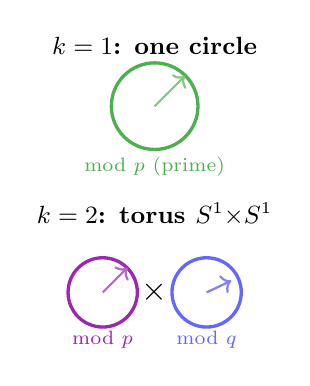
\begin{tikzpicture}[scale=0.55]
  \node[font=\small\bfseries] at (2,6.2) {$k=1$: one circle};
  \draw[always,very thick] (2,4.8) circle (1.0);
  \node[font=\scriptsize,always] at (2,3.4) {mod $p$ (prime)};
  \draw[->,thick,always!70] (2,4.8) -- (2.7,5.5);

  \node[font=\small\bfseries] at (2,2.3) {$k=2$: torus $S^1 {\times} S^1$};

  \draw[vae,very thick] (0.8,0.5) circle (0.8);
  \draw[blue!60,very thick] (3.2,0.5) circle (0.8);
  \node[font=\scriptsize,vae] at (0.8,-0.6) {mod $p$};
  \node[font=\scriptsize,blue!60] at (3.2,-0.6) {mod $q$};
  \draw[->,thick,vae!70] (0.8,0.5) -- (1.37,1.07);
  \draw[->,thick,blue!50] (3.2,0.5) -- (3.77,0.77);
  \node[font=\large] at (2,0.5) {$\times$};
\end{tikzpicture}

\vspace{0.2em}
{\scriptsize Nonlinear methods reveal the manifold's true topology, not its linear embedding dimension.}
\end{column}
\end{columns}
\end{frame}

%% ===================================================================
%% 10c. NLP tasks: Structured pi-SAE on GPT-2 language tasks
%% ===================================================================
\hypertarget{sec10c}{}
\section{10c. Beyond grokking: NLP tasks on GPT-2}

%% --- SLIDE: NLP task results overview ---
\begin{frame}{Structured pi-SAE on GPT-2 language tasks}
\vspace{-0.3em}

\begin{columns}[T]
\begin{column}{0.50\textwidth}
{\small Apply to \textbf{5 NLP tasks} in GPT-2-small, layer 10.}

\vspace{0.2em}
{\scriptsize Using MIB counterfactual pairs (Hanna et al.\ 2024):}
\begin{itemize}\setlength{\itemsep}{0pt}
  \item {\scriptsize \textbf{SVA}: singular/plural agreement (12,400 pairs)}
  \item {\scriptsize \textbf{Greater-than}: year comparison (1,000 pairs)}
  \item {\scriptsize \textbf{Gender bias}: occupation $\to$ he/she (986 pairs)}
  \item {\scriptsize \textbf{Capitals}: country $\to$ capital (190 pairs)}
  \item {\scriptsize \textbf{Hypernymy}: word $\to$ category (198 pairs)}
\end{itemize}

\vspace{0.2em}
{\scriptsize Does pi-SAE's conservatism hold on language tasks?}
\end{column}
\begin{column}{0.48\textwidth}
{\scriptsize\centering
\renewcommand{\arraystretch}{1.05}
\begin{tabular}{l|ccc}
\toprule
\textbf{Task} & \textbf{DAS} & \textbf{NL-DAS} & \textbf{Str.\ pi-SAE} \\
\midrule
\multicolumn{4}{c}{\textit{$k = 1$}} \\
\midrule
SVA        & 0.00 & \textcolor{red}{1.00} & 0.00 \\
Greater-th & 0.03 & \textcolor{red}{1.00} & 0.00 \\
Gender bias& 0.88 & \textcolor{red}{1.00} & 0.54 \\
Capitals   & 0.00 & 0.00 & \textbf{0.12} \\
Hypernymy  & 0.03 & 0.20 & \textbf{0.50} \\
\midrule
\multicolumn{4}{c}{\textit{$k = 4$}} \\
\midrule
SVA        & 0.02 & \textcolor{red}{1.00} & 0.00 \\
Greater-th & 0.31 & \textcolor{red}{1.00} & 0.00 \\
Gender bias& \textbf{1.00} & \textcolor{red}{1.00} & 0.95 \\
Capitals   & 0.02 & 0.07 & \textbf{0.37} \\
Hypernymy  & 0.08 & 0.43 & \textbf{0.47} \\
\bottomrule
\end{tabular}
}

\vspace{0.2em}
{\scriptsize \textcolor{red}{Red}: NL-DAS false positives.}
\end{column}
\end{columns}
\end{frame}

%% --- SLIDE: Three regimes ---
\begin{frame}{Three regimes of causal structure}
\vspace{-0.3em}

\begin{columns}[T]
\begin{column}{0.32\textwidth}
\fcolorbox{neutral}{neutral!8}{\parbox{0.9\linewidth}{\centering\vspace{0.1em}
{\scriptsize\bfseries 1. High-dimensional}\\[0.2em]
{\scriptsize SVA, greater-than}
\vspace{0.1em}}}

\vspace{0.3em}
{\scriptsize All methods except NL-DAS get $\approx 0$.\\[0.2em]
NL-DAS gets $1.0$ = \textcolor{red}{false positive}.\\[0.2em]
Pi-SAE correctly returns 0:\\no low-dim structure exists.}
\end{column}
\begin{column}{0.32\textwidth}
\fcolorbox{always}{always!8}{\parbox{0.9\linewidth}{\centering\vspace{0.1em}
{\scriptsize\bfseries 2. Genuinely low-dim}\\[0.2em]
{\scriptsize Gender bias}
\vspace{0.1em}}}

\vspace{0.3em}
{\scriptsize Binary task (he/she), linearly accessible.\\[0.2em]
DAS: 0.88--1.0.\\
Pi-SAE: 0.54--0.95.\\[0.2em]
Both find it, DAS is slightly better on this linear task.}
\end{column}
\begin{column}{0.32\textwidth}
\fcolorbox{vae}{vae!8}{\parbox{0.9\linewidth}{\centering\vspace{0.1em}
{\scriptsize\bfseries 3. Nonlinear structure}\\[0.2em]
{\scriptsize Capitals, hypernymy}
\vspace{0.1em}}}

\vspace{0.3em}
{\scriptsize DAS fails ($\approx 0$).\\
NL-DAS also weak.\\[0.2em]
\textbf{Pi-SAE is the only method that finds structure.}\\[0.2em]
Capitals: 0.37 at $k{=}4$.\\
Hypernymy: 0.50 at $k{=}1$.}
\end{column}
\end{columns}

\vspace{0.5em}
\centering
\fcolorbox{vae}{vae!8}{\parbox{0.85\textwidth}{\centering\vspace{0.1em}
{\small Pi-SAE is \textbf{conservative}: returns 0 when no structure exists, finds structure where linear methods can't.}
\vspace{0.1em}}}
\end{frame}

%% --- SLIDE: Factorized DAS comparison ---
\begin{frame}{Factorized DAS matches optimal DAS exactly}
\vspace{-0.3em}

\begin{columns}[T]
\begin{column}{0.48\textwidth}
{\small Hard-mode IIA, layer 8, $k{=}1$, atomic-sweep-40:}

\vspace{0.3em}
{\scriptsize\centering
\renewcommand{\arraystretch}{1.1}
\begin{tabular}{l|cc}
\toprule
\textbf{Task} & \textbf{DAS} & \textbf{Fac.\ DAS} \\
\midrule
IOI       & 0.94 & 0.94 \\
SVA       & 0.79 & 0.79 \\
Gender    & 0.79 & 0.83 \\
Capitals  & 0.69 & 0.69 \\
Hypernymy & 1.00 & 1.00 \\
\bottomrule
\end{tabular}
}

\vspace{0.3em}
{\scriptsize Factorized DAS recovers the same subspace as optimal DAS on every task.}
\end{column}
\begin{column}{0.48\textwidth}
{\small \textbf{Complementary tools:}}

\vspace{0.3em}
{\scriptsize
\begin{tabular}{@{}lcc@{}}
\toprule
& \textbf{DAS} & \textbf{Str.\ pi-SAE} \\
\midrule
Linear tasks & \textcolor{always}{\checkmark} & \checkmark \\
Nonlinear    & $\times$ & \textcolor{always}{\checkmark} \\
False positives & low & \textcolor{always}{none} \\
\bottomrule
\end{tabular}
}

\vspace{0.5em}
{\small DAS \textbf{identifies subspaces} (linearly accessible variables).\\[0.2em]
Pi-SAE \textbf{detects structure} (including nonlinear).\\[0.2em]
\textbf{Together}: structure detection + subspace identification.}
\end{column}
\end{columns}
\end{frame}

%% ===================================================================
%% Feature analysis: what do the learned features look like?
%% ===================================================================
\hypertarget{sec_features}{}
\section{What do the features learn?}

%% --- SLIDE: Feature sparsity ---
\begin{frame}{Most features are causally inert}
\vspace{-0.5em}

\begin{columns}[T]
\begin{column}{0.48\textwidth}
\centering
{\small \textbf{Addition} (grokked, 32 features)}

\vspace{0.2em}
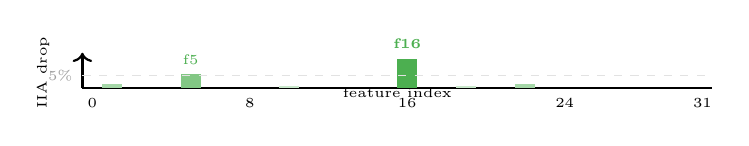
\begin{tikzpicture}[xscale=0.25, yscale=3.2]
  \draw[thick] (0,0) -- (32,0);
  \draw[thick,->] (0,0) -- (0,0.14);
  \node[font=\tiny,rotate=90] at (-2,0.06) {IIA drop};
  \node[font=\tiny] at (16,-0.02) {feature index};

  \fill[always] (16,0) rectangle (17,0.117);
  \fill[always!70] (5,0) rectangle (6,0.056);
  \fill[always!50] (1,0) rectangle (2,0.017);
  \fill[always!50] (22,0) rectangle (23,0.017);
  \fill[always!30] (10,0) rectangle (11,0.006);
  \fill[always!30] (19,0) rectangle (20,0.006);

  \foreach \x in {0,8,16,24,31}
    \node[font=\tiny,below] at (\x+0.5,-0.003) {\x};
  \draw[neutral!30,dashed] (0,0.05) -- (32,0.05);
  \node[font=\tiny,neutral,left] at (0,0.05) {5\%};

  \node[font=\tiny\bfseries,always,above] at (16.5,0.117) {f16};
  \node[font=\tiny,always,above] at (5.5,0.056) {f5};
\end{tikzpicture}

\vspace{0.1em}
{\scriptsize \textbf{3 of 32} features account for 97\% of causal effect.\\
26 features have \textbf{zero} IIA impact when ablated.}
\end{column}
\begin{column}{0.48\textwidth}
\centering
{\small \textbf{Gender bias} (GPT-2, 32 features)}

\vspace{0.2em}
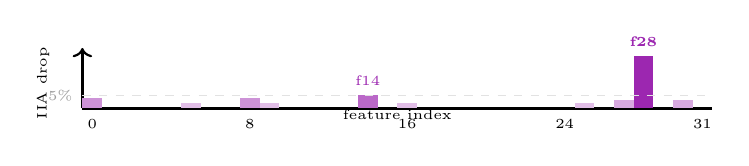
\begin{tikzpicture}[xscale=0.25, yscale=3.2]
  \draw[thick] (0,0) -- (32,0);
  \draw[thick,->] (0,0) -- (0,0.24);
  \node[font=\tiny,rotate=90] at (-2,0.1) {IIA drop};
  \node[font=\tiny] at (16,-0.025) {feature index};

  \fill[vae] (28,0) rectangle (29,0.207);
  \fill[vae!70] (14,0) rectangle (15,0.053);
  \fill[vae!50] (0,0) rectangle (1,0.040);
  \fill[vae!50] (8,0) rectangle (9,0.040);
  \fill[vae!40] (27,0) rectangle (28,0.033);
  \fill[vae!40] (30,0) rectangle (31,0.033);
  \fill[vae!30] (5,0) rectangle (6,0.020);
  \fill[vae!30] (9,0) rectangle (10,0.020);
  \fill[vae!30] (16,0) rectangle (17,0.020);
  \fill[vae!30] (25,0) rectangle (26,0.020);

  \foreach \x in {0,8,16,24,31}
    \node[font=\tiny,below] at (\x+0.5,-0.004) {\x};
  \draw[neutral!30,dashed] (0,0.05) -- (32,0.05);
  \node[font=\tiny,neutral,left] at (0,0.05) {5\%};

  \node[font=\tiny\bfseries,vae,above] at (28.5,0.207) {f28};
  \node[font=\tiny,vae,above] at (14.5,0.053) {f14};
\end{tikzpicture}

\vspace{0.1em}
{\scriptsize \textbf{Feature 28 alone} causes 0.21 IIA drop.\\
Binary task $\to$ one dominant feature (the he/she direction).}
\end{column}
\end{columns}

\vspace{0.3em}
\centering
\fcolorbox{always}{always!8}{\parbox{0.85\textwidth}{\centering\vspace{0.1em}
{\small Sparse features are \textbf{genuinely sparse}. Ablation reveals which carry causal information and which are inert.}
\vspace{0.1em}}}
\end{frame}

%% --- SLIDE: Fourier alignment ---
\begin{frame}{Grokking features align with Fourier modes}
\vspace{-0.5em}

\begin{columns}[T]
\begin{column}{0.50\textwidth}
{\small For addition mod 113, all 32 features align to \textbf{frequency 9}:}

\vspace{0.2em}
{\scriptsize\centering
\renewcommand{\arraystretch}{1.0}
\begin{tabular}{@{}lccl@{}}
\toprule
& \textbf{$\rho$} & \textbf{Freq.} & \textbf{Component} \\
\midrule
f16 (rank 1) & \textbf{0.55} & 9 & $\cos$ \\
f19           & \textbf{0.58} & 9 & $\cos$ \\
f1 (rank 3)   & 0.48 & 9 & $\sin$ \\
f15           & 0.48 & 9 & $\sin$ \\
f11           & 0.43 & 9 & $\sin$ \\
f6            & 0.39 & 9 & $\sin$ \\
\midrule
\multicolumn{4}{c}{\textit{31 of 32 features: frequency 9}} \\
\bottomrule
\end{tabular}
}

\vspace{0.3em}
{\scriptsize Confirms Nanda et al.\ (2023): grokked addition uses Fourier components of $s = (a{+}b) \bmod 113$.\\[0.2em]
The pi-SAE \textbf{rediscovers} this without being told about Fourier modes.}
\end{column}
\begin{column}{0.48\textwidth}
\centering
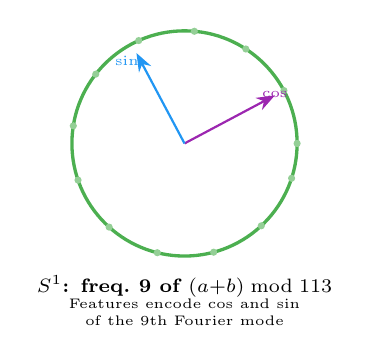
\begin{tikzpicture}[scale=0.65]
  \draw[always,very thick] (0,0) circle (2.2);

  \foreach \angle in {0, 28, 57, 85, 114, 142, 171, 199, 228, 256, 285, 313, 342} {
    \fill[always!60] ({2.2*cos(\angle)},{2.2*sin(\angle)}) circle (2pt);
  }

  \draw[vae,thick,-{Stealth}] (0,0) -- ({2.0*cos(28)},{2.0*sin(28)});
  \node[font=\tiny,vae,above right] at ({1.5*cos(28)},{1.5*sin(28)}) {$\cos$};
  \draw[das,thick,-{Stealth}] (0,0) -- ({2.0*cos(118)},{2.0*sin(118)});
  \node[font=\tiny,das,above left] at ({1.5*cos(118)},{1.5*sin(118)}) {$\sin$};

  \node[font=\scriptsize\bfseries] at (0,-2.8) {$S^1$: freq.\ 9 of $(a{+}b) \bmod 113$};
  \node[font=\tiny,align=center] at (0,-3.3) {Features encode cos and sin\\of the 9th Fourier mode};
\end{tikzpicture}

\vspace{0.3em}
\fcolorbox{neutral}{neutral!8}{\parbox{0.9\linewidth}{\centering\vspace{0.1em}
{\scriptsize \textbf{Multiplication}: Fourier $\rho < 0.03$.\\Multiplicative structure $\neq$ clean Fourier modes.}
\vspace{0.1em}}}
\end{column}
\end{columns}
\end{frame}

%% --- SLIDE: Max-activating examples ---
\begin{frame}{What do the features detect? Max-activating examples}
\vspace{-0.5em}

\begin{columns}[T]
\begin{column}{0.48\textwidth}
{\small\textbf{Gender bias: feature 28} (dominant, IIA drop: \textbf{0.21})}

\vspace{0.2em}
{\scriptsize
\renewcommand{\arraystretch}{1.1}
\begin{tabular}{@{}r l@{}}
\toprule
\textbf{Act.} & \textbf{Text} \\
\midrule
\textcolor{das}{+3.59} & The \textbf{assassin} wanted that \\
\textcolor{das}{+3.49} & The \textbf{collector} was promoted because \\
\textcolor{das}{+3.44} & The \textbf{tutor} yelled that \\
\midrule
\textcolor{circle}{$-$3.43} & The \textbf{actress} was promoted because \\
\textcolor{circle}{$-$3.43} & The \textbf{performer} yelled that \\
\textcolor{circle}{$-$3.43} & The \textbf{teenager} ate because \\
\bottomrule
\end{tabular}
}

\vspace{0.2em}
{\scriptsize \textcolor{das}{Positive}: male-stereotyped occupations.\\
\textcolor{circle}{Negative}: female-stereotyped occupations.\\[0.1em]
\textbf{Feature 28 is the gender direction.}}
\end{column}
\begin{column}{0.48\textwidth}
{\small\textbf{Hypernymy: distributed features}}

\vspace{0.2em}
{\scriptsize
\renewcommand{\arraystretch}{1.0}
\begin{tabular}{@{}lcc@{}}
\toprule
\textbf{Feature} & \textbf{IIA drop} & \textbf{Role} \\
\midrule
f8  & 0.167 & primary \\
f4  & 0.100 & secondary \\
f10 & 0.083 & secondary \\
f1  & 0.050 & tertiary \\
f6  & 0.050 & tertiary \\
\midrule
\multicolumn{3}{c}{\textit{20 of 32 features contribute}} \\
\bottomrule
\end{tabular}
}

\vspace{0.3em}
\centering
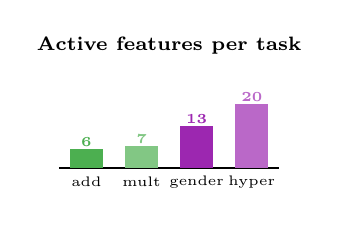
\begin{tikzpicture}[xscale=0.70,yscale=1.3]
  \node[font=\scriptsize\bfseries] at (2,1.2) {Active features per task};
  \draw[thick] (0,0) -- (4,0);

  \fill[always] (0.2,0) rectangle (0.8,0.19);
  \node[font=\tiny] at (0.5,-0.13) {add};
  \node[font=\tiny\bfseries,always] at (0.5,0.26) {6};

  \fill[always!70] (1.2,0) rectangle (1.8,0.22);
  \node[font=\tiny] at (1.5,-0.13) {mult};
  \node[font=\tiny\bfseries,always!70] at (1.5,0.29) {7};

  \fill[vae] (2.2,0) rectangle (2.8,0.41);
  \node[font=\tiny] at (2.5,-0.13) {gender};
  \node[font=\tiny\bfseries,vae] at (2.5,0.48) {13};

  \fill[vae!70] (3.2,0) rectangle (3.8,0.63);
  \node[font=\tiny] at (3.5,-0.13) {hyper};
  \node[font=\tiny\bfseries,vae!70] at (3.5,0.70) {20};
\end{tikzpicture}
\end{column}
\end{columns}

\vspace{0.2em}
\centering
\fcolorbox{vae}{vae!8}{\parbox{0.85\textwidth}{\centering\vspace{0.1em}
{\small Grokking: \textbf{few features, high sparsity}. NLP: \textbf{more features, distributed}. The pi-SAE adapts to each task's intrinsic complexity.}
\vspace{0.1em}}}
\end{frame}

%% --- SLIDE: E2E intervention training results ---
\begin{frame}{End-to-end intervention training: the breakthrough}

\begin{columns}[T]
\begin{column}{0.48\textwidth}
{\small \textbf{Key insight}: train Structured pi-SAE with \textbf{differentiable intervention CE loss} --- backprop through the model's own logits after intervention.}

\vspace{0.3em}
{\small Two-phase training:}
\begin{enumerate}
  \item {\small Warmup (200 epochs): reconstruction + classification only}
  \item {\small E2E (300 epochs): add $-\log p(\text{src\_token} \mid \text{intervened})$}
\end{enumerate}

\vspace{0.3em}
{\small This is what DAS does implicitly --- train on the intervention objective. But we combine it with \textbf{structured sparsity} and \textbf{nonlinear} encoding.}

\vspace{0.5em}
{\small \textbf{Result}: Structured pi-SAE E2E achieves \textbf{0.97 standard IIA} on hypernymy ($k{=}1$), where DAS gets 0.07.}

\vspace{0.3em}
{\small $14\times$ better than DAS, $1.35\times$ better than nonlinear DAS.}
\end{column}
\begin{column}{0.50\textwidth}
{\scriptsize\centering
\renewcommand{\arraystretch}{1.15}
\textbf{Hypernymy --- standard IIA (strict IIA)}\\[0.3em]
\begin{tabular}{l|cc}
\toprule
\textbf{Method} & \textbf{$k = 1$} & \textbf{$k = 4$} \\
\midrule
DAS              & 0.07 (0.02) & 0.23 (0.08) \\
NL-DAS           & 0.72 (0.15) & 0.92 (0.32) \\
\midrule
Vanilla VAE      & 0.00 (0.00) & 0.48 (0.18) \\
pi-VAE           & 0.00 (0.00) & 0.57 (0.20) \\
Str.\ pi-SAE     & 0.58 (0.17) & 0.52 (0.13) \\
\midrule
\textbf{Str.\ pi-SAE E2E} & \textbf{0.97 (0.90)} & \textbf{0.98 (0.85)} \\
\bottomrule
\end{tabular}
}

\vspace{0.5em}
{\scriptsize\centering
\textbf{Gender bias --- standard IIA (strict IIA)}\\[0.3em]
\begin{tabular}{l|cc}
\toprule
\textbf{Method} & \textbf{$k = 1$} & \textbf{$k = 4$} \\
\midrule
DAS              & 0.62 (0.51) & 0.88 (0.85) \\
NL-DAS           & 1.00 (1.00) & 1.00 (1.00) \\
\midrule
Str.\ pi-SAE     & 0.41 (0.35) & 0.52 (0.46) \\
\textit{Str.\ pi-SAE E2E} & \textit{pending} & \textit{pending} \\
\bottomrule
\end{tabular}
}

\vspace{0.3em}
{\scriptsize All results: additive intervention, layer 8.}
\end{column}
\end{columns}
\end{frame}

%% --- SLIDE: E2E why it works ---
\begin{frame}{Why E2E works: closing the training-evaluation gap}

\begin{columns}[T]
\begin{column}{0.50\textwidth}
\textbf{Without E2E} (classification loss only):
\begin{itemize}
  \item {\small Encoder learns to classify labels}
  \item {\small Decoder learns to reconstruct activations}
  \item {\small But: \textbf{swapping $z_c$} and decoding may produce activations the model doesn't interpret correctly}
  \item {\small Reconstruction error $\neq$ intervention error}
\end{itemize}

\vspace{0.5em}
\textbf{With E2E} (intervention CE loss):
\begin{itemize}
  \item {\small Encoder/decoder jointly optimized so that \textbf{swapped codes produce correct model outputs}}
  \item {\small The model itself is the judge}
  \item {\small Additive intervention: $h' = h + \text{dec}(z_{\text{swap}}) - \text{dec}(z_{\text{orig}})$}
  \item {\small Reconstruction errors cancel out}
\end{itemize}
\end{column}
\begin{column}{0.48\textwidth}

\vspace{0.3em}
{\scriptsize \textbf{Additive vs.\ replacement intervention:}}

\vspace{0.2em}
{\scriptsize\centering
\setlength{\tabcolsep}{3pt}
\renewcommand{\arraystretch}{1.0}
\begin{tabular}{@{}l|cc@{}}
\toprule
\textbf{Hypernymy $k{=}1$} & \textbf{Add.} & \textbf{Repl.} \\
\midrule
Str.\ pi-SAE     & 0.58 & 0.60 \\
Str.\ pi-SAE E2E & \textbf{0.97} & \textbf{0.97} \\
\midrule
\textbf{Strict IIA} & & \\
\midrule
Str.\ pi-SAE     & 0.17 & 0.18 \\
Str.\ pi-SAE E2E & \textbf{0.90} & \textbf{0.88} \\
\bottomrule
\end{tabular}
}

\vspace{0.4em}
{\small E2E training eliminates the gap between additive and replacement --- the decoder learns to produce activations the model actually uses.}

\vspace{0.3em}
{\small \textbf{Key}: E2E + structured sparsity is the combination. E2E alone (on vanilla VAE) would overfit; sparsity constrains the causal subspace.}
\end{column}
\end{columns}
\end{frame}

\hypertarget{sec11}{}
\section{11. Cross-task transfer}

%% --- SLIDE: Cross-task transfer on IOI ---
\begin{frame}{Cross-task transfer validates causal variables}

\begin{columns}[T]
\begin{column}{0.55\textwidth}
{\small A genuine causal variable should \textbf{transfer} --- train on one task variant, test on another.}

\vspace{0.3em}
{\small \textbf{IOI cross-template transfer} (GPT-2):}
\begin{itemize}
  \item {\small Train VAE on templates 1--3}
  \item {\small Test on unseen templates 4--5}
  \item {\small IIA = 0.82--0.96 at $k = 4$}
\end{itemize}

\vspace{0.3em}
{\small \textbf{Extended IOI tasks}\footnote{\tiny Nainani et al., arXiv:2411.16105, 2024.}:}
\begin{itemize}
  \item {\small DoubleIO: IIA = 0.77--0.81}
  \item {\small TripleIO: IIA = 0.77--0.81}
  \item {\small Trained only on base IOI!}
\end{itemize}

\end{column}
\begin{column}{0.42\textwidth}
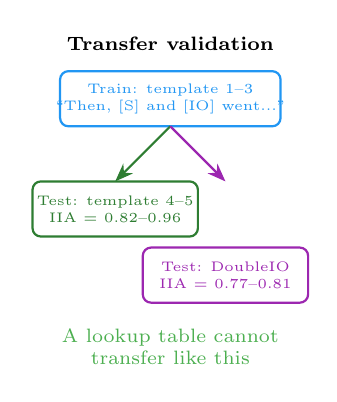
\begin{tikzpicture}[scale=0.7]
  % Transfer diagram
  \node[font=\scriptsize\bfseries] at (0,5.0) {Transfer validation};

  % Train
  \draw[das,thick,rounded corners=3pt] (-2,3.5) rectangle (2,4.5);
  \node[font=\tiny,das,align=center] at (0,4.0) {Train: template 1--3\\``Then, [S] and [IO] went...''};

  % Test 1
  \draw[grass,thick,-{Stealth}] (0,3.5) -- (-1,2.5);
  \draw[grass,thick,rounded corners=3pt] (-2.5,1.5) rectangle (0.5,2.5);
  \node[font=\tiny,grass,align=center] at (-1,2.0) {Test: template 4--5\\IIA = 0.82--0.96};

  % Test 2
  \draw[vae,thick,-{Stealth}] (0,3.5) -- (1,2.5);
  \draw[vae,thick,rounded corners=3pt] (-0.5,0.3) rectangle (2.5,1.3);
  \node[font=\tiny,vae,align=center] at (1,0.8) {Test: DoubleIO\\IIA = 0.77--0.81};

  % The point
  \node[font=\scriptsize,pass,align=center] at (0,-0.5) {A lookup table cannot\\transfer like this};
\end{tikzpicture}

\vspace{0.3em}
{\scriptsize \textbf{IOI subtask transfer}\footnote{\tiny Prakash et al., ICLR 2024 (MIB).} (8 types):}\\
{\scriptsize DAS ratio: 0.56 ~$\cdot$~ VAE ratio: 0.43}
\end{column}
\end{columns}
\end{frame}

%% --- SLIDE: Cross-task IIA transfer matrix ---
\begin{frame}{Cross-task transfer: train on A, evaluate on B}

\begin{columns}[T]
\begin{column}{0.50\textwidth}
{\scriptsize Train Structured pi-SAE on one task, freeze encoder/decoder, evaluate IIA on a different task's counterfactual pairs.}

\vspace{0.3em}
{\scriptsize \textbf{IIA transfer matrix} ($k{=}4$, layer 8, additive):}

\vspace{0.2em}
{\scriptsize\centering
\setlength{\tabcolsep}{3pt}
\renewcommand{\arraystretch}{1.05}
\begin{tabular}{@{}l|ccc@{}}
\toprule
\textbf{Train $\backslash$ Eval} & \textbf{Gender} & \textbf{Hyper.} & \textbf{Gt.} \\
\midrule
Gender bias  & \textbf{1.00} & 0.00 & 0.41 \\
Hypernymy    & 0.30 & \textbf{0.98} & 0.43 \\
Greater-than & 0.31 & 0.00 & \textbf{1.00} \\
\bottomrule
\end{tabular}
}

\vspace{0.3em}
{\scriptsize \textbf{Findings}:}
\begin{itemize}\setlength{\itemsep}{1pt}
  \item {\scriptsize Gender $\leftrightarrow$ greater-than: partial transfer ($\sim$0.3--0.4)}
  \item {\scriptsize Hypernymy is isolated --- 0.0 transfer with gender}
  \item {\scriptsize Diagonal dominates: task-specific structure is real}
\end{itemize}
\end{column}
\begin{column}{0.48\textwidth}
{\scriptsize \textbf{Subspace geometry}:}

\vspace{0.2em}
{\scriptsize\centering
\setlength{\tabcolsep}{3pt}
\renewcommand{\arraystretch}{1.05}
\begin{tabular}{@{}l|cc@{}}
\toprule
\textbf{Task pair} & \textbf{cos $\theta$} & \textbf{$d_G$} \\
\midrule
Gender--Hyper.  & 0.11 & 2.92 \\
Gender--Gt.     & 0.09 & 2.96 \\
Hyper.--Gt.     & 0.09 & 2.96 \\
\bottomrule
\end{tabular}
}

\vspace{0.3em}
{\scriptsize Grassmannian distance $d_G \approx 2.9$. The decoder causal subspaces are \textbf{nearly orthogonal}.}

\vspace{0.3em}
{\scriptsize \textbf{Interpretation}: each task occupies its own region of the residual stream. Partial transfer (gender $\leftrightarrow$ greater-than) comes from \textbf{shared numerical structure}, not shared subspaces.}

\vspace{0.3em}
{\scriptsize Consistent with superposition --- GPT-2 packs many independent causal variables into the same residual stream.}
\end{column}
\end{columns}
\end{frame}

%% --- SLIDE: Feature composition - DAS vs pi-SAE ---
\begin{frame}{Feature composition: DAS vs.\ pi-SAE}

\begin{columns}[T]
\begin{column}{0.50\textwidth}
\textbf{DAS: direction arithmetic}

\vspace{0.3em}
{\small Linear DAS learns a rotation $Q$ per task. To compose:}
\begin{itemize}
  \item {\small $h' = h + Q_A^\top z_A + Q_B^\top z_B$ (add both)}
  \item {\small $h' = h - Q_A^\top z_A$ (negate A)}
\end{itemize}

\vspace{0.3em}
{\small Problems:}
\begin{itemize}
  \item {\small Directions may not be orthogonal}
  \item {\small Adding two continuous rotations can interfere}
  \item {\small Only works if structure is linear}
\end{itemize}
\end{column}
\begin{column}{0.48\textwidth}
\textbf{Structured pi-SAE: feature switching}

\vspace{0.3em}
{\small Each sparse feature is an independent binary knob:}
\begin{itemize}
  \item {\small Activate features 3 and 7: both effects}
  \item {\small Zero feature 5: negate that effect}
  \item {\small Set feature 3 to specific value: titrated control}
\end{itemize}

\vspace{0.3em}
{\small Sparsity guarantees near-independence by construction.}
\end{column}
\end{columns}

\vspace{0.5em}
\centering
\fcolorbox{grass}{grass!8}{\parbox{0.85\textwidth}{\centering\vspace{0.1em}
{\small Sparse features compose without interference. Continuous directions do not.}
\vspace{0.1em}}}
\end{frame}

%% --- SLIDE: Feature composition - diagram ---
\begin{frame}{Sparse features as independent causal knobs}

\centering
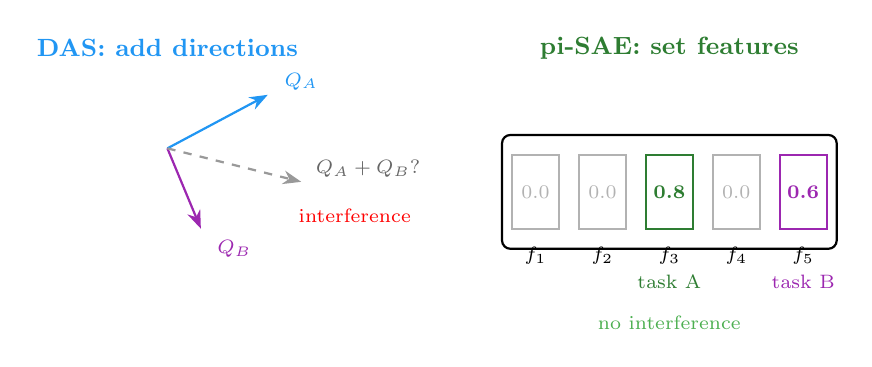
\begin{tikzpicture}[scale=0.85]
  % DAS side
  \node[font=\small\bfseries,das] at (-4,4.5) {DAS: add directions};
  \draw[das,thick,-{Stealth}] (-4,3.0) -- (-2.5,3.8);
  \node[font=\scriptsize,das] at (-2.0,4.0) {$Q_A$};
  \draw[vae,thick,-{Stealth}] (-4,3.0) -- (-3.5,1.8);
  \node[font=\scriptsize,vae] at (-3.0,1.5) {$Q_B$};
  \draw[black!40,thick,dashed,-{Stealth}] (-4,3.0) -- (-2.0,2.5);
  \node[font=\scriptsize,black!60] at (-1.0,2.7) {$Q_A + Q_B$?};
  \node[font=\scriptsize,red] at (-1.2,2.0) {interference};

  % SAE side
  \node[font=\small\bfseries,grass] at (3.5,4.5) {pi-SAE: set features};
  \draw[thick,rounded corners=3pt] (1.0,1.5) rectangle (6.0,3.2);

  % Feature slots
  \foreach \x/\lab/\val/\col in {1.5/1/0.0/black!30, 2.5/2/0.0/black!30, 3.5/3/\textbf{0.8}/grass, 4.5/4/0.0/black!30, 5.5/5/\textbf{0.6}/vae} {
    \draw[\col,thick] (\x-0.35,1.8) rectangle (\x+0.35,2.9);
    \node[font=\scriptsize,\col] at (\x,2.35) {\val};
    \node[font=\scriptsize] at (\x,1.4) {$f_{\lab}$};
  }
  \node[font=\scriptsize,grass] at (3.5,1.0) {task A};
  \node[font=\scriptsize,vae] at (5.5,1.0) {task B};
  \node[font=\scriptsize,pass] at (3.5,0.4) {no interference};
\end{tikzpicture}

\vspace{0.5em}
{\small \textbf{Next}: train pi-SAE on tasks A and B, compose by setting features from both, measure joint IIA.}\\[0.2em]
{\small If causal features are truly independent, composition should ``just work.''}
\end{frame}

\hypertarget{sec13}{}
\section{13. Four-level hierarchy}

%% --- SLIDE: The hierarchy ---
\begin{frame}{A four-level hierarchy for causal validity}

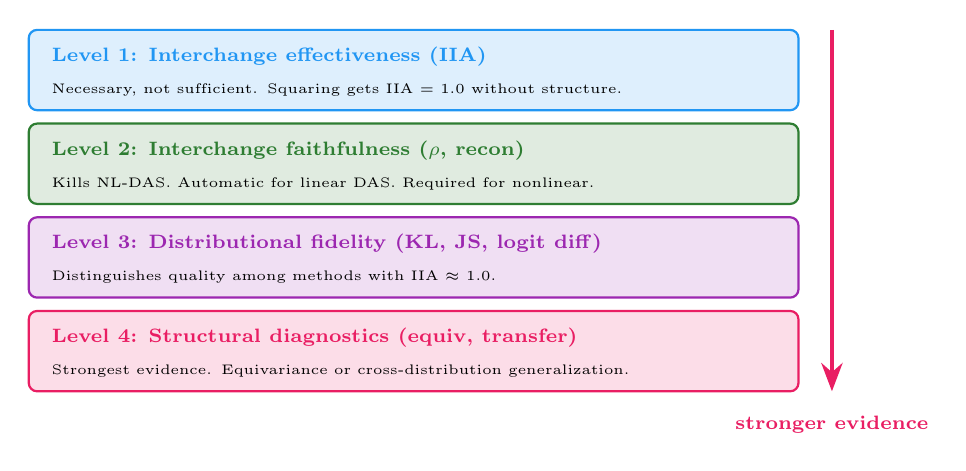
\begin{tikzpicture}[scale=0.85]
  % Level 1
  \fill[das!15,rounded corners=3pt] (-5.5,3.2) rectangle (6,4.4);
  \draw[das,thick,rounded corners=3pt] (-5.5,3.2) rectangle (6,4.4);
  \node[font=\scriptsize\bfseries,das,anchor=west] at (-5.3,4.0) {Level 1: Interchange effectiveness (IIA)};
  \node[font=\tiny,anchor=west,text width=10.8cm] at (-5.3,3.5) {Necessary, not sufficient. Squaring gets IIA = 1.0 without structure.};

  % Level 2
  \fill[grass!15,rounded corners=3pt] (-5.5,1.8) rectangle (6,3.0);
  \draw[grass,thick,rounded corners=3pt] (-5.5,1.8) rectangle (6,3.0);
  \node[font=\scriptsize\bfseries,grass,anchor=west] at (-5.3,2.6) {Level 2: Interchange faithfulness ($\rho$, recon)};
  \node[font=\tiny,anchor=west,text width=10.8cm] at (-5.3,2.1) {Kills NL-DAS. Automatic for linear DAS. Required for nonlinear.};

  % Level 3
  \fill[vae!15,rounded corners=3pt] (-5.5,0.4) rectangle (6,1.6);
  \draw[vae,thick,rounded corners=3pt] (-5.5,0.4) rectangle (6,1.6);
  \node[font=\scriptsize\bfseries,vae,anchor=west] at (-5.3,1.2) {Level 3: Distributional fidelity (KL, JS, logit diff)};
  \node[font=\tiny,anchor=west,text width=10.8cm] at (-5.3,0.7) {Distinguishes quality among methods with IIA $\approx$ 1.0.};

  % Level 4
  \fill[circle!15,rounded corners=3pt] (-5.5,-1.0) rectangle (6,0.2);
  \draw[circle,thick,rounded corners=3pt] (-5.5,-1.0) rectangle (6,0.2);
  \node[font=\scriptsize\bfseries,circle,anchor=west] at (-5.3,-0.2) {Level 4: Structural diagnostics (equiv, transfer)};
  \node[font=\tiny,anchor=west,text width=10.8cm] at (-5.3,-0.7) {Strongest evidence. Equivariance or cross-distribution generalization.};

  % Strength arrow
  \draw[circle,ultra thick,-{Stealth}] (6.5,4.4) -- (6.5,-1.0);
  \node[font=\scriptsize\bfseries,circle] at (6.5,-1.5) {stronger evidence};
\end{tikzpicture}

\vspace{0.5em}
{\small \textbf{Key asymmetry}: Linear DAS automatically passes Level 2 (orthogonal projection is faithful by construction) but may fail Level 1 on nonlinear variables. NL-DAS easily passes Level 1 but fails Level 2.}
\end{frame}

\hypertarget{sec14}{}
\section{14. Continuous metrics}

%% --- SLIDE: Binary vs continuous ---
\begin{frame}{Binary IIA hides important differences}

\begin{columns}[T]
\begin{column}{0.48\textwidth}
\centering
\textbf{Binary IIA}

\vspace{0.3em}
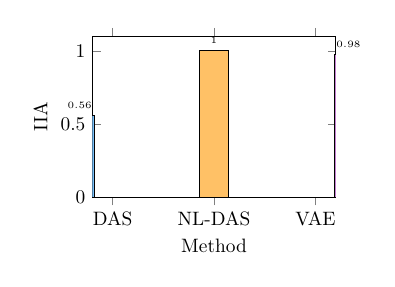
\begin{tikzpicture}[scale=0.7]
  \begin{axis}[
    width=6cm, height=4.5cm,
    ybar,
    bar width=15pt,
    xlabel={Method},
    ylabel={IIA},
    ymin=0, ymax=1.1,
    xtick={1,2,3},
    xticklabels={DAS,NL-DAS,VAE},
    ytick={0,0.5,1.0},
    nodes near coords,
    every node near coord/.append style={font=\tiny},
  ]
  \addplot[fill=das!60] coordinates {(1,0.556)};
  \addplot[fill=nldas!60] coordinates {(2,1.000)};
  \addplot[fill=vae!60] coordinates {(3,0.978)};
  \end{axis}
\end{tikzpicture}

{\small NL-DAS ``wins.'' But it is a lookup table.}
\end{column}
\begin{column}{0.48\textwidth}
\centering
\textbf{With faithfulness metrics}

\vspace{0.3em}
{\small\setlength{\tabcolsep}{2pt}
\begin{tabular}{lccc}
\toprule
& \textbf{DAS} & \textbf{NL-DAS} & \textbf{VAE} \\
\midrule
IIA & 0.556 & \textcolor{fail}{1.000} & \textcolor{pass}{0.978} \\
Diversity $\rho$ & 1.0 & \textcolor{fail}{$\approx 0$} & \textcolor{pass}{$\approx 1$} \\
Transfer & Yes & \textcolor{fail}{No} & \textcolor{pass}{Yes} \\
\bottomrule
\end{tabular}}

\vspace{0.5em}
{\small VAE wins genuinely. NL-DAS is disqualified by $\rho \approx 0$.}

\vspace{0.3em}
{\small DAS is honest but limited by linearity.}
\end{column}
\end{columns}
\end{frame}

\hypertarget{sec15}{}
\section{15. Practical advice}

%% --- SLIDE: Practical advice ---
\begin{frame}{Our flowchart for causal abstraction}
\vspace{-0.3em}

\begin{enumerate}\setlength{\itemsep}{2pt}
  \item {\scriptsize \textbf{Never report IIA alone.} IIA = 1.0 is compatible with genuine structure, memorized lookup tables, and degenerate encoder-decoders. Always report at least one faithfulness metric.}

  \item {\scriptsize \textbf{Use continuous distributional metrics.} KL divergence and normalized logit difference distinguish among methods that all achieve IIA $\approx 1.0$. Binary IIA treats a 51\% shift the same as 99\%.}

  \item {\scriptsize \textbf{Be suspicious of unconstrained nonlinear featurizers.} Any encoder-decoder trained end-to-end on interchange loss without reconstruction constraints can learn a lookup table. The ELBO (or equivalent) is necessary.}

  \item {\scriptsize \textbf{Test cross-distribution generalization.} Evaluate on disjoint names, novel templates, or new task variants. A method that fails under distribution shift is exploiting surface regularities.}

  \item {\scriptsize \textbf{Consider nonlinear methods when DAS IIA is low.} Low IIA does not mean no causal variable --- it may mean DAS is searching the wrong function class. But validate with faithfulness metrics.}
\end{enumerate}
\end{frame}

%% --- SLIDE: Surprising cases ---
\begin{frame}{Surprising positive and negative cases}

\begin{columns}[T]
\begin{column}{0.48\textwidth}
\textbf{\textcolor{pass}{Surprising positives}}

\vspace{0.3em}
{\small \textbf{Cubic sum} ($a^3 + b^3$): perfect equivariance (100\%) despite cubing alone reaching only 50.9\%. The boundary is not ``group action vs.\ polynomial'' but whether the binary structure provides sufficient additive symmetry.}

\vspace{0.5em}
{\small \textbf{Max} ($\max(a,b)$): achieves 95.7\% equivariance despite not being a group action. It is piecewise equivariant: when the argmax is stable under shift, max behaves like a shifted identity.}
\end{column}
\begin{column}{0.48\textwidth}
\textbf{\textcolor{fail}{Surprising negatives}}

\vspace{0.3em}
{\small \textbf{Affine} ($2a + 3b + 5$): a \emph{linear} function that \emph{fails} to produce a Grassmannian variable! Under $a \mapsto a + g$, the output shifts by $2g$, not $g$. Equivariance requires the operation to be a group action, not merely linear.}

\vspace{0.5em}
{\small \textbf{Squaring}: achieves IIA = 1.0 by $k = 4$ without grokking. High IIA is the illusion; low equivariance (31.4\%) is the truth.}
\end{column}
\end{columns}
\end{frame}

\hypertarget{sec16}{}
\section{16. Conclusions}

%% --- SLIDE: Conclusions ---
\begin{frame}{Conclusions}
\vspace{-0.3em}

\begin{enumerate}\setlength{\itemsep}{6pt}
  \item {\small 14 operations $\to$ three sharp classes (Always / Stochastic / Never Grassmannian). Boundary governed by grokking.}

  \item {\small Linear DAS returns IIA $= 0$ on grokked addition. The variable lives on $S^1$, not $\Gr(k,d)$. Category error.}

  \item {\small Unconstrained NL-DAS achieves IIA $= 1.0$ vacuously (lookup table). Diversity ratio $\rho$ exposes this.}

  \item {\small Structured VAE recovers genuine nonlinear causal variables. ELBO prevents degeneracy. Transfers across tasks.}
\end{enumerate}

\vspace{0.5em}
{\small The linearity assumption is \textbf{testable}. The natural fix (nonlinearity) introduces a new failure mode. This paper provides the diagnostics to detect both problems and the method to avoid them.}
\end{frame}

%% --- SLIDE: The big picture ---
\begin{frame}{Summary}
\vspace{-0.5em}

\centering
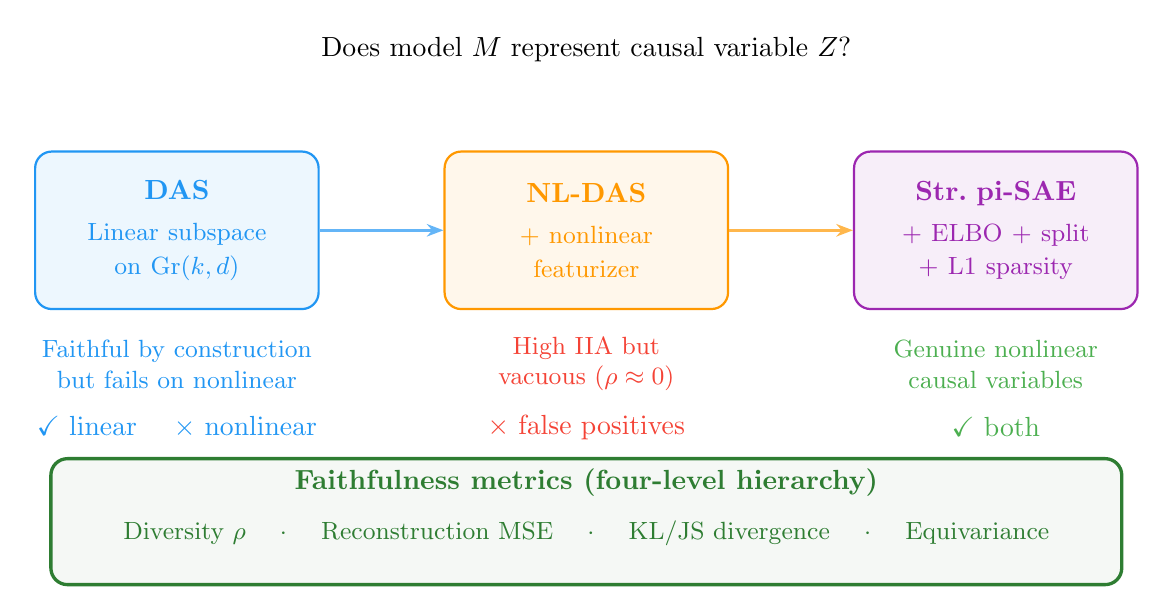
\begin{tikzpicture}[
  method/.style={thick, rounded corners=6pt, minimum width=3.6cm, minimum height=2.0cm, align=center, draw, text width=3.2cm},
  label/.style={font=\small, align=center},
  arr/.style={very thick, -{Stealth[length=6pt]}}
]
  % The problem
  \node[font=\normalsize, align=center] at (0, 4.5) {Does model $M$ represent causal variable $Z$?};

  % Three methods as a progression — spread wider
  \node[method, das, fill=das!8] (das) at (-5.2, 2.2) {
    \textbf{\normalsize DAS}\\[0.3em]
    {\small Linear subspace}\\
    {\small on $\Gr(k,d)$}
  };

  \node[method, nldas, fill=nldas!8] (nldas) at (0, 2.2) {
    \textbf{\normalsize NL-DAS}\\[0.3em]
    {\small + nonlinear}\\
    {\small featurizer}
  };

  \node[method, vae, fill=vae!8] (vae) at (5.2, 2.2) {
    \textbf{\normalsize Str.\ pi-SAE}\\[0.3em]
    {\small + ELBO + split}\\
    {\small + L1 sparsity}
  };

  % Arrows between methods
  \draw[arr, das!70] (das) -- (nldas);
  \draw[arr, nldas!70] (nldas) -- (vae);

  % Verdicts below each
  \node[label, das] at (-5.2, 0.5) {Faithful by construction\\but fails on nonlinear};
  \node[label, never] at (0, 0.5) {High IIA but\\vacuous ($\rho \approx 0$)};
  \node[label, always] at (5.2, 0.5) {Genuine nonlinear\\causal variables};

  % Checkmarks / X marks
  \node[font=\normalsize, das] at (-5.2, -0.3) {\checkmark\ linear \quad $\times$\ nonlinear};
  \node[font=\normalsize, never] at (0, -0.3) {$\times$\ false positives};
  \node[font=\normalsize, always] at (5.2, -0.3) {\checkmark\ both};

  % Faithfulness metrics box spanning full width
  \draw[grass, very thick, rounded corners=6pt, fill=grass!5] (-6.8, -2.3) rectangle (6.8, -0.7);
  \node[font=\normalsize\bfseries, grass] at (0, -1.0) {Faithfulness metrics (four-level hierarchy)};
  \node[font=\small, grass] at (0, -1.65) {Diversity $\rho$ \quad $\cdot$ \quad Reconstruction MSE \quad $\cdot$ \quad KL/JS divergence \quad $\cdot$ \quad Equivariance};
\end{tikzpicture}

\vspace{0.2em}
{\scriptsize IIA is necessary but never sufficient. Every causal abstraction claim needs the \textbf{four-level hierarchy}.}
\end{frame}

%% --- SLIDE: Thank you ---
\begin{frame}[plain]
\vfill
\begin{center}
{\Large\bfseries Thank you}

\vspace{1em}
{\small Elliot Tower}

\vspace{1em}
{\small Code and experiments:\\
\texttt{github.com/elliottower/grokking-causal-geometry}}

\vspace{1em}
{\small Draft paper: \emph{When Does Linear Causal Abstraction Work?\\Mapping the Boundary on the Grassmannian}}
\end{center}
\vfill
\end{frame}

\end{document}
